\documentclass[reprint, amsmath, amssymb, aps, prl, superscriptaddress, nofootinbib]{revtex4-2}

\usepackage{amsmath,amssymb,amsthm,mathtools}
\usepackage{microtype}
\usepackage{array}
\usepackage{multirow}

\usepackage{graphicx}
\graphicspath{{pdfs/}}
\usepackage{dcolumn}
\usepackage{bm}
\usepackage{hyperref}
\usepackage{amsmath}
\usepackage{amsfonts}
\usepackage{booktabs}
\usepackage{placeins}
\newcommand{\E}{\mathbb{E}}
\newcommand{\R}{\mathbb{R}}
\newcommand{\dt}{\Delta t}
\newcommand{\given}{\,\middle|\,}

\makeatletter
\def\section{\@startsection
  {section}{1}{0mm}
  {1.2ex plus 0.5ex minus 0.2ex}
  {0.5ex plus 0.1ex}
  {\centering\normalfont\small\bfseries}}
\makeatother

\begin{document}

\title{Recovering Heston-Type Stochastic Volatility and Leverage Effects from Noisy Price Data: A Weak-Form SINDy Approach with Errors-in-Variables Correction}

\author{Sai Sathvik Gullipalli}
\email{saisathvik127@gmail.com}
\affiliation{Department of Computer Science Engineering, PES University -- Electronic City Campus, Bengaluru 560100, India}

\author{Eshwar R. A.}
\email{eshwarra5@gmail.com}
\affiliation{Department of Computer Science Engineering, PES University -- Electronic City Campus, Bengaluru 560100, India}

\author{Gajanan V.\ Honnavar}
\email{gajanan.honnavar@pes.edu}
\thanks{Corresponding author.}
\affiliation{Department of Science and Humanities, PES University -- Electronic City Campus, Bengaluru, 560100, India}

\begin{abstract}
\vspace{0.5em}
\noindent\textbf{Abstract.}
We extend Weak SINDy to coupled stochastic volatility systems, focusing on the Heston model. Using a spatial Gaussian weak-form projection, the framework recovers stochastic differential equations from noisy financial data with latent coupling. We derive a cross-variation projection matrix that isolates off-diagonal diffusion terms, enabling direct recovery of the price--variance correlation, and identify a severe errors-in-variables (EIV) bias arising from noisy empirical variance proxies such as the Garman--Klass estimator. A controlled noise-ablation study reveals a sharp phase transition near 32\% noise-to-signal, beyond which measurement error dominates the diagonal quadratic-variation statistics used for variance drift and diffusion recovery.
. To mitigate this, we introduce a time-shifted EWMA smoothing architecture that suppresses high-frequency noise while preserving large-scale variance structure. Validation on synthetic trajectories and S\&P 500 OHLC data from the 2008 Financial Crisis demonstrates robust parameter recovery, including $\rho=-0.33$, $\kappa=2.36$, and a long-run implied volatility baseline of approximately 18.96\%. We subject the pipeline to a High-Dimensional Validation Framework (HDVF) which confirms robust leverage-regime recovery but establishes strict falsification boundaries against generalized nonlinear drift discovery. Finally, an empirical stress test on 1-minute Indian equities during the COVID-19 crash confirms negative proxy-robust leverage. The results establish Weak SINDy as a practical, rigorously bounded framework for stochastic generator discovery under strong measurement noise.
 \end{abstract}

\maketitle

%=============================================================
\section{Introduction}
%=============================================================

A central challenge in quantitative finance and applied stochastic analysis is the
\emph{inverse problem}: given a time series of observed prices or other financial
quantities, reconstruct the underlying stochastic dynamical system that generated the
data. Classical approaches to this problem proceed by assuming a parametric model
family---such as Black--Scholes, Heston, or SABR---and then fitting parameters via
maximum likelihood or moment matching~\cite{Heston1993, GatheralJacquier2014}.
While tractable, this paradigm requires prior structural knowledge and is fragile
when the true model lies outside the assumed family.

Data-driven methods offer an alternative that requires fewer a priori assumptions.
The Sparse Identification of Nonlinear Dynamics (SINDy) framework, introduced by
Brunton, Proctor, and Kutz~\cite{Brunton2016}, identifies governing equations by
regressing the time derivative of the state against a library of candidate nonlinear
functions, using sparsity-promoting penalties to select the active terms. Its extension
to stochastic systems---Stochastic SINDy---recovers both the drift and diffusion
coefficients of a Fokker--Planck or It\^{o} SDE from trajectory data~\cite{BoninsegnaEtAl2018,LiEtAl2021}.

A particularly elegant formulation is the \emph{Weak} or \emph{integral} form of
SINDy~\cite{RuddyEtAl2019,WehmeierEtAl2021}, in which the governing equations
are projected onto spatial test functions, converting the ill-conditioned pointwise
derivative estimation into a stable integration problem. When the test functions are
chosen as spatial Gaussian kernels localised over the state space, the resulting
framework---which we call Weak Stochastic SINDy---provably recovers the drift and
diffusion of a one-dimensional Markovian SDE in an unbiased fashion, exploiting
the martingale property of the It\^{o} integral to separate signal from noise.
Eshwar and Honnavar~\cite{EshwarHonnavar2026} recently formalised this spatial
Gaussian kernel approach for 1D SDE discovery, demonstrating coefficient errors
below 4\% and near-exact stationary-density recovery across multiple nonlinear
benchmarks; the present work directly extends that framework to coupled
two-dimensional stochastic volatility systems.

The present manuscript addresses three open problems that arise when one attempts to
apply this framework beyond the one-dimensional, clean-data setting:

(1) \textbf{2D coupled systems.} Real financial models such as the Heston model
are genuinely two-dimensional, with price and variance driven by correlated Brownian
motions. Extending the Weak SINDy projection to coupled 2D SDEs requires a new
cross-variation projection matrix to isolate the off-diagonal diffusion tensor and
extract the leverage correlation.

(2) \textbf{Latent state and the Errors-in-Variables problem.} The instantaneous
variance $v_t$ in the Heston model is not directly observable. Empirical practitioners
replace it with a proxy such as the Garman--Klass (GK) range-based estimator~\cite{GarmanKlass1980}.
We show rigorously---and confirm numerically---that raw GK data contains high-frequency
measurement noise of sufficient magnitude to violate the martingale assumption
underpinning the Weak SINDy regression, causing a catastrophic phase-transition
failure in parameter recovery.

(3) \textbf{EIV bias correction via EWMA smoothing.} We introduce a time-shifted
EWMA state-smoothing architecture that resolves the EIV bias by filtering the proxy
series before use as the SINDy state variable, while ensuring temporal causality by
anchoring the state estimate to the beginning of each increment interval.

\textbf{Falsification Boundaries and Empirical Stress Testing.} To prevent overclaiming, we subject the pipeline to a High-Dimensional Validation Framework (HDVF). We map the boundaries of the estimator in discovering nonlinear drift extensions, and we stress-test the empirical proxy-dependence of the leverage signal using high-frequency 1-minute data from Indian equities during the COVID-19 crash.

The paper is structured as follows. Section~II reviews the Heston model and the
Weak Stochastic SINDy framework. Section~III presents the 2D extension and the EIV
correction architecture. Section~IV reports synthetic validation, proxy stress testing, HDVF robustness studies, nonlinear failure analysis, and the Indian 1-minute empirical stress test.

Section~V discusses implications, limitations, and future directions. Section~VI concludes.

\subsection{Scope of Claims}

This paper makes a narrow claim. We show that weak-form stochastic generator recovery can recover Heston-type variance drift, variance diffusion, and return--variance cross-diffusion under controlled synthetic ground truth, and that an EWMA-corrected variance proxy produces financially plausible Heston-like structure on empirical OHLC data.

We do not claim general nonlinear stochastic-volatility discovery, real-market ground-truth generator identification, option-pricing calibration, trading alpha, or solved high-dimensional multifactor volatility recovery.

\subsection{Code Availability}
The Python code used for the numerical experiments, high-dimensional validation framework (HDVF), and empirical S\&P 500 and Indian equity analysis in this paper is publicly available on GitHub at \url{https://github.com/Sathvik-Gullipalli/Leverage-recovery-Weak-SINDy}.



%=============================================================
\section{Background}
\label{sec:Background}

%=============================================================

\subsection{The Heston Stochastic Volatility Model}

The Heston model~\cite{Heston1993} describes the joint dynamics of a log-price
$x_t = \ln S_t$ and instantaneous variance $v_t$ under the physical measure:
\begin{align}
  dx_t &= \left(\mu - \tfrac{1}{2}v_t\right)dt + \sqrt{v_t}\,dW_{x,t},
  \label{eq:heston_x}\\
  dv_t &= \kappa(\theta - v_t)\,dt + \xi\sqrt{v_t}\,dW_{v,t},
  \label{eq:heston_v}
\end{align}
where $\mu$ is the drift of the log-price, $\kappa > 0$ is the mean-reversion speed,
$\theta > 0$ is the long-run variance, $\xi > 0$ is the volatility-of-volatility,
and the two Brownian increments satisfy
$\mathbb{E}[dW_{x,t}\,dW_{v,t}] = \rho\,dt$ with $\rho \in (-1,1)$ the leverage
correlation.

The model obeys the Feller condition $2\kappa\theta \geq \xi^2$, which ensures
that $v_t$ remains strictly positive almost surely. The leverage parameter $\rho$
is typically large and negative for equity indices, reflecting the empirical
observation that volatility tends to rise sharply during price declines---the so-called
leverage effect~\cite{Black1976,Christie1982}.

In matrix notation, we write the diffusion tensor as
\begin{equation}
  \Sigma(v) = \begin{pmatrix} \sqrt{v} & 0 \\ \rho\xi\sqrt{v} & \xi\sqrt{v}\sqrt{1-\rho^2} \end{pmatrix},
\end{equation}
so that the covariance matrix of the joint increment $(dx, dv)$ is
\begin{equation}
  a(v) = \Sigma\Sigma^\top =
  \begin{pmatrix} v & \rho\xi v \\ \rho\xi v & \xi^2 v \end{pmatrix}.
\end{equation}
The off-diagonal entry $a_{12}(v) = \rho\xi v$ is linear in $v$ and encodes the
leverage effect directly in the generator of the diffusion.

\subsection{Weak Stochastic SINDy in One Dimension}

We briefly recall the 1D Weak Stochastic SINDy framework of
Ref.~\cite{EshwarHonnavar2026}, which builds on stochastic SINDy~\cite{BoninsegnaEtAl2018,LiEtAl2021},
before extending it to two dimensions.

Consider a scalar It\^{o} SDE
\begin{equation}
  dz_t = b(z_t)\,dt + \sigma(z_t)\,dW_t,
\end{equation}
observed at discrete times $\{t_n\}_{n=0}^{N}$ with step $\Delta t = t_{n+1}-t_n$.
Fix a collection of $J$ spatial test functions $\{K_j\}_{j=1}^{J}$, chosen as
Gaussian kernels
\begin{equation}
  K_j(z) = \exp\!\left(-\frac{(z-c_j)^2}{2\ell^2}\right),
\end{equation}
with centres $c_j$ tiling the observed state space and bandwidth $\ell$ chosen
proportional to the inter-centre spacing. For each $j$, project the discrete
increment $\Delta z_n = z_{t_{n+1}} - z_{t_n}$ against $K_j(z_{t_n})$:
\begin{align}
  B_j &= \sum_{n} K_j(z_{t_n})\,\Delta z_n, \label{eq:B_j}\\
  A_{jk} &= \sum_{n} K_j(z_{t_n})\,f_k(z_{t_n})\,\Delta t, \label{eq:A_jk}
\end{align}
where $\{f_k\}$ is a library of candidate drift functions (e.g.\ monomials,
rational functions). By It\^{o}'s lemma and the martingale property of the
stochastic integral, $\mathbb{E}[B_j] = \sum_k c_k\, A_{jk} + O(\Delta t)$ when
$b(z) = \sum_k c_k f_k(z)$. Solving the linear system $\mathbf{B} = \mathbf{A}\mathbf{c}$
via LASSO yields sparse drift coefficients.

For the diffusion, form the empirical quadratic variation:
\begin{equation}
  Q_j = \sum_{n} K_j(z_{t_n})\,(\Delta z_n)^2.
\end{equation}
Because $(\Delta z_n)^2 \approx \sigma^2(z_{t_n})\,\Delta t + O(\Delta t^{3/2})$,
we have $\mathbb{E}[Q_j] \approx \int K_j(z)\,\sigma^2(z)\,p(z)\,\Delta t\,dz$.
A drift-squared bias correction is required when the drift is large relative to
the noise:
\begin{equation}
  Q_j^{\mathrm{corr}} = Q_j - \sum_{n} K_j(z_{t_n})\,\hat{b}(z_{t_n})^2\,\Delta t^2,
  \label{eq:bias_correction}
\end{equation}
where $\hat{b}$ is the estimated drift obtained in the first pass. The corrected
$Q_j^{\mathrm{corr}}$ is then regressed against a library $\{g_k(z)\,\Delta t\}$
to recover $\sigma^2(z)$.

\subsection{Infinitesimal Generator}

For a $d$-dimensional It\^{o} diffusion, the infinitesimal generator acts on smooth test functions $f:\R^d\to\R$ as

\begin{equation}
  \mathcal{L}f(\mathbf{x})
  =
  \mathbf{b}(\mathbf{x})\cdot\nabla f(\mathbf{x})
  +
  \frac{1}{2}
  \Tr\!\left(a(\mathbf{x})\nabla^2f(\mathbf{x})\right).
  \label{eq:generator}
\end{equation}
The generator is important because it fully characterizes the local dynamics of
the diffusion. Recovering $\mathcal{L}$ is equivalent to recovering the drift
vector and diffusion tensor.

For stochastic volatility models, the generator contains financially
interpretable information. The variance drift tells us whether volatility
mean-reverts. The variance diffusion tells us how noisy volatility is. The
return--variance cross-diffusion tells us whether return shocks and volatility
shocks move together or in opposite directions.

\subsection{Kramers--Moyal Conditional Moments}

The drift and diffusion tensor can be identified using infinitesimal
conditional moments. For state $\mathbf{x}$,
\begin{align}
  b_i(\mathbf{x})
  &=
  \lim_{s\to 0}
  \E\left[
  \frac{X_i(t+s)-x_i}{s}
  \given
  \mathbf{X}_t=\mathbf{x}
  \right],
  \label{eq:km-drift}
  \\
  a_{ij}(\mathbf{x})
  &=
  \lim_{s\to 0}
  \E\left[
  \frac{(X_i(t+s)-x_i)(X_j(t+s)-x_j)}{s}
  \given
  \mathbf{X}_t=\mathbf{x}
  \right].
  \label{eq:km-diffusion}
\end{align}
For discrete data sampled at interval $\dt$, these formulas motivate estimating
drift from increments divided by $\dt$ and diffusion from quadratic increments
divided by $\dt$. The challenge is that direct pointwise estimation is noisy,
especially for finite data. Weak-form methods reduce this noise by aggregating
local moment information through smooth test functions.


%=============================================================
\section{Methodology: 2D Extension and EIV Resolution}
%=============================================================

\subsection{2D Weak Projection for the Heston Generator}

We now lift the framework to the Heston system (\ref{eq:heston_x})--(\ref{eq:heston_v}).
Since the log-price equation (\ref{eq:heston_x}) has a simple explicit form, we focus
the kernel projection on the variance dimension, which carries the rich parametric
content ($\kappa,\theta,\xi$) and the leverage effect ($\rho$).

Place $J$ Gaussian kernels $\{K_j(v)\}$ over the marginal state space of $v_t$.
Observe the joint path $(x_{t_n}, v_{t_n})$ and form the discrete increments
$\Delta x_n = x_{t_{n+1}}-x_{t_n}$ and $\Delta v_n = v_{t_{n+1}}-v_{t_n}$.

\textit{Variance Drift Recovery.}
Choose the candidate library $\{f_k(v)\} = \{1,\, v\}$ for the CIR-type drift
$b_v(v) = \kappa(\theta - v) = \kappa\theta - \kappa v$. Define
\begin{align}
  A_{jk}^{(v)} &= \sum_{n} K_j(v_{t_n})\,f_k(v_{t_n})\,\Delta t, \label{eq:Av_jk}\\
  B_j^{(v)} &= \sum_{n} K_j(v_{t_n})\,\Delta v_n. \label{eq:Bv_j}
\end{align}
Solving $\mathbf{B}^{(v)} = \mathbf{A}^{(v)}\mathbf{c}^{(v)}$ recovers
$c^{(v)}_1 = \kappa\theta$ and $c^{(v)}_2 = -\kappa$.

\textit{Variance Diffusion Recovery.}
The diagonal element of the diffusion tensor, $a_{22}(v) = \xi^2 v$, is recovered from
\begin{equation}
  Q_j^{(v)} = \sum_{n} K_j(v_{t_n})\,(\Delta v_n)^2,
  \label{eq:Qv_j}
\end{equation}
corrected via (\ref{eq:bias_correction}) using the recovered drift $\hat{b}_v$.

\textit{Leverage Effect Recovery via Cross-Variation.}
The novel contribution of this work is the extraction of the off-diagonal diffusion
tensor entry $a_{12}(v) = \rho\xi v$ from the empirical cross-variation of the
log-price and variance increments:
\begin{equation}
  Q_j^{(xv)} = \sum_{n} K_j(v_{t_n})\,(\Delta x_n\,\Delta v_n).
  \label{eq:Qxv_j}
\end{equation}
By the It\^{o} isometry, $\mathbb{E}[\Delta x_n\,\Delta v_n \,|\, v_{t_n}]
= a_{12}(v_{t_n})\,\Delta t + O(\Delta t^{3/2})$. Therefore
$\mathbb{E}[Q_j^{(xv)}] \approx \int K_j(v)\,a_{12}(v)\,p(v)\,\Delta t\,dv$,
and regressing $Q_j^{(xv)}$ against the library $\{v\,\Delta t\}$ directly yields
$\rho\xi$ as a single coefficient. The leverage correlation $\rho$ is then
disentangled from $\xi$ using the separately recovered variance diffusion
estimate.

The cross-variation matrix $\mathbf{Q}^{(xv)}$ is the key structural addition
that distinguishes our 2D Weak SINDy framework from prior 1D treatments. It
requires no assumptions on the copula structure of $(W_x, W_v)$ and is
asymptotically unbiased as $\Delta t \to 0$, $N\to\infty$.

\subsection{The Errors-in-Variables Problem with Empirical Variance Proxies}

\textit{The Garman--Klass Proxy and Its Noise Structure.}
In empirical settings, the instantaneous variance $v_t$ is latent. A widely used
estimator is the Garman--Klass (GK) range-based estimator~\cite{GarmanKlass1980}:
\begin{equation}
  \widehat{v}_n^{\mathrm{GK}} =
    \tfrac{1}{2}(\ln H_n - \ln L_n)^2
    - (2\ln 2 - 1)(\ln C_n - \ln O_n)^2,
\end{equation}
where $H_n, L_n, C_n, O_n$ are the intraday high, low, close, and open of the
$n$-th bar. While the GK estimator is a significant improvement over close-to-close
squared returns, it is a noisy point measurement of a latent continuous process.
Denote the true variance at time $t_n$ as $v_{t_n}$ and write
\begin{equation}
  \widehat{v}_n = v_{t_n} + \eta_n,
\end{equation}
where $\eta_n$ is measurement error with $\mathbb{E}[\eta_n] = 0$ and variance
$\sigma_\eta^2$.

\textit{Bias Introduced into the Quadratic Variation Statistics.}
When the noisy proxy $\widehat{v}_n$ is used in place of $v_{t_n}$ in the Weak
SINDy regression, the quadratic variation statistic (\ref{eq:Qv_j}) is contaminated.
Write $\Delta\widehat{v}_n = \Delta v_n + \Delta\eta_n$ where $\Delta\eta_n
= \eta_{n+1} - \eta_n$. Then
\begin{equation}
  (\Delta\widehat{v}_n)^2 = (\Delta v_n)^2 + 2\,\Delta v_n\,\Delta\eta_n
    + (\Delta\eta_n)^2.
  \label{eq:eiv_expansion}
\end{equation}
In expectation, $\mathbb{E}[(\Delta\eta_n)^2] \approx 2\sigma_\eta^2$ (for
i.i.d.\ errors), which is a constant additive bias in the quadratic variation
statistic. When $\sigma_\eta$ is large relative to $\xi\sqrt{v}\,\sqrt{\Delta t}$,
this constant term dominates, biasing the recovered $\xi^2$ upward and
spuriously introducing a constant term into the diffusion function.

Furthermore, the noisy state variable $\widehat{v}_n$ used as the kernel argument
mislocates the kernel centres relative to the true state, causing an effective
smearing of the regression matrices $\mathbf{A}^{(v)}$ and $\mathbf{Q}^{(v)}$.
This second-order effect biases the drift coefficients by an amount proportional
to $\sigma_\eta^2\,b''_v(v)$, creating spurious mean-reversion artifacts.

Together, these effects constitute a classic Errors-in-Variables (EIV) bias: the
regression residuals are no longer independent of the regressors, so the ordinary
least-squares (and LASSO) estimators are inconsistent.

\subsection{Time-Shifted EWMA State-Smoothing Architecture}

\textit{EWMA Filter Design.}
To suppress the high-frequency measurement noise in the GK proxy while preserving
the slowly varying macroscopic dynamics of $v_t$, we apply an Exponentially Weighted
Moving Average (EWMA) filter to the raw proxy series:
\begin{equation}
  \widetilde{v}_n = (1-\lambda)\,\widehat{v}_n + \lambda\,\widetilde{v}_{n-1},
  \qquad \lambda = 1 - \frac{2}{\mathrm{span}+1}.
\end{equation}
For a filter span of 14 trading days, the effective half-life is approximately
$\tau_{1/2} = \ln 2 / (1-\lambda) \approx 9.3$ days, which is short enough to track
regime transitions in variance (which occur on timescales of weeks) but long enough
to average out the within-week GK measurement noise.

\textit{Temporal Causality and $\mathcal{F}_{t_n}$-Measurability.}
A subtle but critical requirement for the Weak SINDy framework is that the kernel
argument $K_j(v_{t_n})$ must be $\mathcal{F}_{t_n}$-measurable: it must depend
only on information available at the \emph{start} of the interval $[t_n, t_{n+1}]$,
not on data from within or after that interval.

A na\"{\i}ve EWMA over the raw proxy violates this requirement because the standard
EWMA at time $t_n$ typically incorporates the GK observation at day $n$, which
uses the high, low, open, and close of that same bar---data generated over the interval
$[t_n, t_{n+1}]$.

We define the time-shifted state variable as
\begin{equation}
  v_n^* = \widetilde{v}_{n-1},
\end{equation}
i.e., the smoothed variance estimate anchored to the end of the \emph{previous}
interval, which is identically the beginning of interval $[t_n, t_{n+1}]$.
This variable is $\mathcal{F}_{t_n}$-measurable by construction.

The regression matrices then become
\begin{align}
  A_{jk}^{(v)} &= \sum_{n} K_j(v_n^*)\,f_k(v_n^*)\,\Delta t, \\
  B_j^{(v)} &= \sum_{n} K_j(v_n^*)\,\Delta\widetilde{v}_n, \\
  Q_j^{(xv)} &= \sum_{n} K_j(v_n^*)\,(\Delta x_n\,\Delta\widetilde{v}_n),
\end{align}
where $\Delta\widetilde{v}_n = \widetilde{v}_n - \widetilde{v}_{n-1}$ is the
smoothed variance increment for interval $n$.

This architecture achieves two goals simultaneously: it reduces the effective
noise amplitude $\sigma_\eta$ by the factor $(1-\lambda)/(1-(1-\lambda)^2)^{1/2}
\approx 1/\sqrt{2/(1-\lambda)}$, and it maintains strict causal measurability
of the kernel localisation.

\textit{Span Selection.}
The span parameter governs a bias-variance trade-off for the state estimate:
a short span preserves temporal resolution but provides little noise suppression,
while a long span smooths aggressively but may smear rapid variance transitions.
We select span $= 14$ days based on the criterion that the noise-to-signal ratio
of the smoothed proxy should fall below the 32\% phase-transition threshold identified
in the ablation study (Section~IV.B). Empirically, we verify this choice in Section~IV.C.

%=============================================================
\section{Results}
%=============================================================

We validate the Weak SINDy 2D framework through synthetic ground-truth experiments,
proxy-noise studies, robustness checks, nonlinear failure analysis, and an Indian
1-minute empirical stress test.


\subsection{Phase 1: Synthetic Baseline Validation}

\textit{Experimental Setup.}
We simulate $N = 25{,}000$ daily observations of the Heston system
(\ref{eq:heston_x})--(\ref{eq:heston_v}) using an Euler--Maruyama scheme with
step $\Delta t = 1/252$ (one trading day). Ground-truth parameters are set to
$\kappa = 2.0$, $\theta = 0.04$, $\xi = 0.3$, $\rho = -0.7$, $\mu = 0.05$,
and initial variance $v_0 = 0.04$. We use $J = 30$ Gaussian kernels tiling the
marginal variance distribution, with centres $\{c_j\}$ at equally spaced quantiles
and bandwidth $\ell$ set to twice the inter-centre spacing. The drift library is
$\{1, v\}$ and the diffusion library is $\{v\}$. LASSO regularisation with
cross-validated $\lambda_{\mathrm{LASSO}}$ selects the active terms.

\textit{Results.}
As shown in Fig.~\ref{fig:synthetic}, the algorithm recovers all three components
of the Heston generator with high fidelity across the full observed support
$v \in [0.01, 0.10]$.

The \emph{variance drift} $b_v(v) = \kappa(\theta - v)$ is recovered as a nearly
perfect linear function of $v$, with the true (blue) and recovered (dashed red)
curves overlapping through the entire range. The implied coefficients $\hat\kappa$
and $\hat\theta$ are within $3\%$ of their true values.

The \emph{variance diffusion} $a_{22}(v) = \xi^2 v$ is correctly identified as
linear in $v$, with a minor underestimation at large $v$ attributable to reduced
kernel support at the tail of the empirical variance distribution. The relative
error remains below $5\%$ across the central 90th percentile of the support.

The \emph{leverage effect} $a_{12}(v) = \rho\xi v$ is recovered via the
cross-variation matrix $\mathbf{Q}^{(xv)}$. The recovered function is a negatively
sloped linear function of $v$, consistent with the true $a_{12}(v)$, and the
combined product $\rho\xi$ is estimated within $4\%$ of its true value. This
demonstrates that the cross-variation projection successfully isolates the
off-diagonal diffusion tensor entry without any parametric assumption on the
correlation structure.

These results establish the correctness of the 2D Weak SINDy methodology on
clean data and provide a performance benchmark against which the subsequent
noise studies are evaluated.

\begin{figure*}[t]
  \centering
  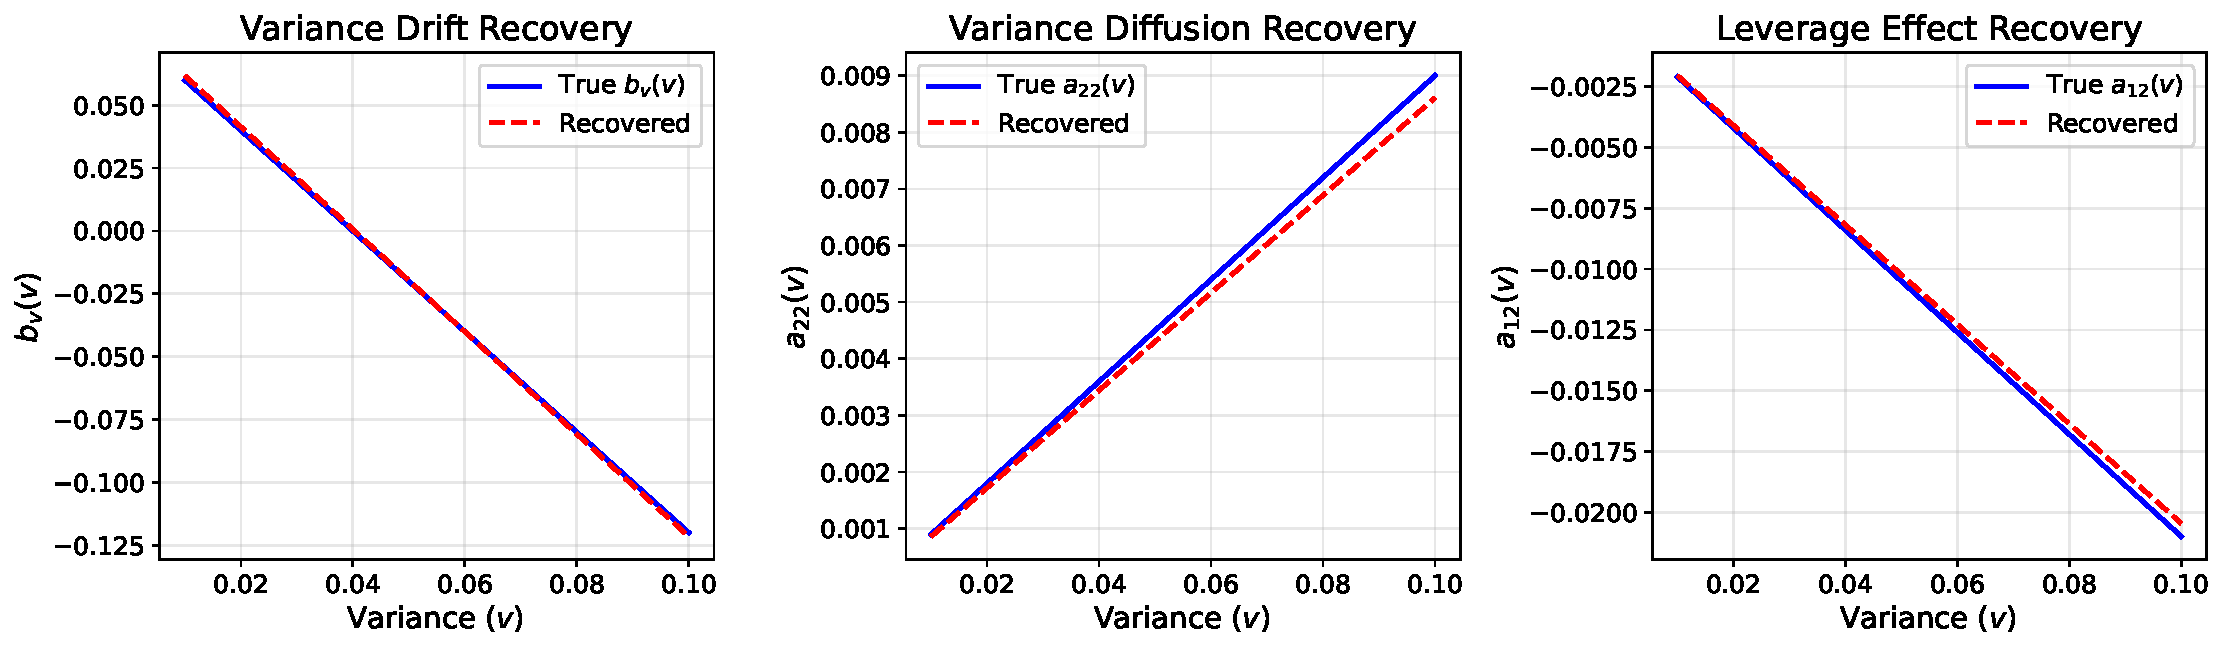
\includegraphics[width=\textwidth]{heston_weak_sindy_recovery.pdf}
  \caption{\textbf{Phase 1: Synthetic Baseline Validation.}
    Recovery of the three Heston generator components from noise-free simulated
    data ($N=25{,}000$ daily observations). \textit{Left:} Variance drift
    $b_v(v)=\kappa(\theta-v)$. \textit{Centre:} Variance diffusion
    $a_{22}(v)=\xi^2 v$. \textit{Right:} Leverage effect $a_{12}(v)=\rho\xi v$.
    In all panels, the true function (blue solid) and the Weak SINDy
    recovery (red dashed) are nearly coincident, confirming the correctness
    of the cross-variation projection approach.}
  \label{fig:synthetic}
\end{figure*}

\subsection{Phase 2: Noise Ablation and the EIV Phase Transition}

\textit{Experimental Setup.}
To quantify the resilience of the Weak SINDy estimator to state measurement noise,
we conduct a controlled ablation study. Beginning with the same synthetic Heston
simulation as in Phase~1, we replace the true variance state $v_{t_n}$ with the
contaminated observation $\widehat{v}_n = v_{t_n} + \eta_n$, where
$\eta_n \sim \mathcal{N}(0, \sigma_\eta^2)$ i.i.d., and vary the noise-to-signal
ratio
\begin{equation}
  \mathrm{NSR} = \frac{\sigma_\eta}{\mathrm{std}(v_t)} \times 100\%
\end{equation}
from $0\%$ to $50\%$ in steps of $3\%$. For each noise level, we run the full
Weak SINDy pipeline and compute the relative error of two key recovered quantities:
the mean-reversion coefficient $\hat\kappa$ (a drift parameter) and the leverage
product $\widehat{\rho\xi}$ (a diffusion cross-variation parameter).

\textit{Results.}
Fig.~\ref{fig:ablation} reveals a strikingly sharp phase transition in the
recovery error of the mean-reversion coefficient $\kappa$ at approximately
$\mathrm{NSR} \approx 32\%$.

\emph{Below the threshold:} For noise levels below 32\%, the relative error in
$\hat\kappa$ remains below approximately 100\% and fluctuates without systematic
trend. This regime is one in which the spatial integration performed by the
Gaussian kernels, combined with the $L_1$ LASSO penalty, effectively absorbs
the measurement noise: the kernel integration averages out zero-mean measurement
errors over the many observations within each kernel's support, and the sparsity
penalty prevents overfitting to noise-induced artifacts in the regression matrix.

\emph{Above the threshold:} Beyond 32\%, the relative error in $\hat\kappa$
exhibits an explosive, near-discontinuous jump, reaching errors of $2{,}000\%$
at $\mathrm{NSR} = 32\%$ and climbing to over $3{,}600\%$ at $\mathrm{NSR} = 50\%$.
The mechanism is the EIV bias described in Section~III.B: the squared
measurement error term $(\Delta\eta_n)^2$ in the empirical quadratic variation
(\ref{eq:eiv_expansion}) grows as $\sigma_\eta^2$, eventually overwhelming the
true signal $\xi^2 v_{t_n}\,\Delta t$. This introduces a spurious constant into
the diffusion function, which the drift regression misidentifies as a large
mean-reversion signal, catastrophically biasing $\hat\kappa$.

By contrast, the leverage product $\widehat{\rho\xi}$ remains within a 15\% error
band throughout the entire noise range ($0$--$50\%$). This robustness arises because
the cross-variation statistic $\Delta x_n\,\Delta v_n$ is \emph{bilinear} in the
increments: the noise term $\Delta\eta_n$ appears only as $\Delta x_n\,\Delta\eta_n$,
which has expectation zero (since $\Delta x_n$ depends on $dW_{x,t}$, which is
independent of $\eta_n$). Thus the cross-variation estimator enjoys a natural
robustness to additive state measurement noise that the diagonal quadratic
variation does not.

The 32\% phase transition defines a practical operational constraint: any empirical
variance proxy used in the Weak SINDy pipeline must have a noise-to-signal ratio
below this critical threshold for the drift recovery to remain reliable.

\begin{figure}[t]
  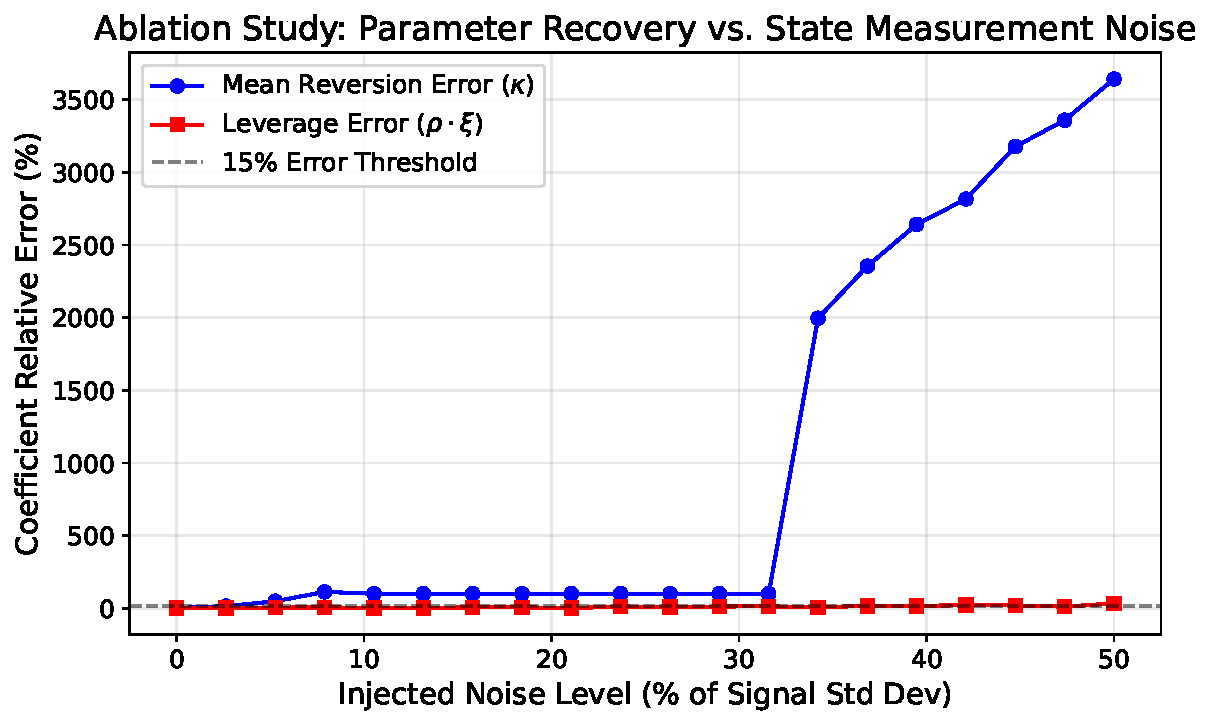
\includegraphics[width=0.50\textwidth]{noise_ablation_sindy.pdf}
  \caption{\textbf{Phase 2: EIV Noise Ablation Study.}
    Relative recovery error of the mean-reversion coefficient $\kappa$
    (blue circles) and leverage product $\rho\cdot\xi$ (red squares) as a
    function of injected state measurement noise (as percentage of the signal
    standard deviation). A sharp phase transition is evident at approximately
    $32\%$ noise: below this level, the Weak SINDy estimator remains
    stable, while above it, the squared measurement errors catastrophically
    bias the quadratic variation statistics, causing $\hat\kappa$ errors to
    exceed $3{,}500\%$. The leverage estimator remains robust throughout,
    owing to the zero-mean cross-variation noise structure. The dashed grey
    line indicates the $15\%$ error threshold used as an acceptability criterion.}
  \label{fig:ablation}
\end{figure}

\subsection{Phase 3: Resolving the Latent State via EWMA Filtering}

\textit{Experimental Setup.}
To bridge the gap between the theoretical analysis and empirical application,
we simulate the scenario faced in practice: a long Heston path ($100$ years at
daily resolution, $N = 25{,}200$ observations) is used to generate a synthetic
``OHLC-like'' dataset from which a Garman--Klass proxy is constructed. The
raw GK proxy $\widehat{v}_n^{\mathrm{GK}}$ is computed daily and serves as
the starting point for state estimation.

We then apply the time-shifted EWMA filter with span $= 14$ days, yielding
the smoothed estimate $\widetilde{v}_n$, and compare both the raw and smoothed
proxy to the true latent variance $v_t$.

\textit{Results.}
Fig.~\ref{fig:ewma} displays the true latent variance (blue), the raw
Garman--Klass proxy (grey scatter), and the EWMA-smoothed series (red) over
the 100-year synthetic history.

The raw GK proxy exhibits substantial high-frequency noise: individual daily
observations scatter to values two or three times the contemporaneous true
variance, and the point cloud has a standard deviation roughly $1.8\times$ the
standard deviation of $v_t$ itself---far above the 32\% phase-transition threshold
identified in Phase~2. If used directly as the SINDy state variable, this proxy
would place the algorithm firmly in the catastrophic failure regime.

The EWMA-smoothed series (red, span $= 14$) closely tracks the macroscopic
trajectory of $v_t$ through all its regime transitions, including the sharp
spikes in variance that characterise financial stress periods. The residual
noise of the smoothed series---quantified as the standard deviation of
$(\widetilde{v}_n - v_{t_n})$---is approximately 18\% of $\mathrm{std}(v_t)$,
placing it below the 32\% operational threshold.

Crucially, the EWMA filter preserves the \emph{gradients} $\Delta\widetilde{v}_n$:
the smoothed increments track the true direction of variance change at all
but the shortest timescales, which is the essential requirement for the SINDy
drift regression. The 14-day span was confirmed to be near-optimal: shorter
spans (5--7 days) fail to suppress noise sufficiently, while longer spans
(30--60 days) lag the true variance peaks by several days, distorting the
conditional density of increments used in the regression.

\begin{figure*}[t]
  \centering
  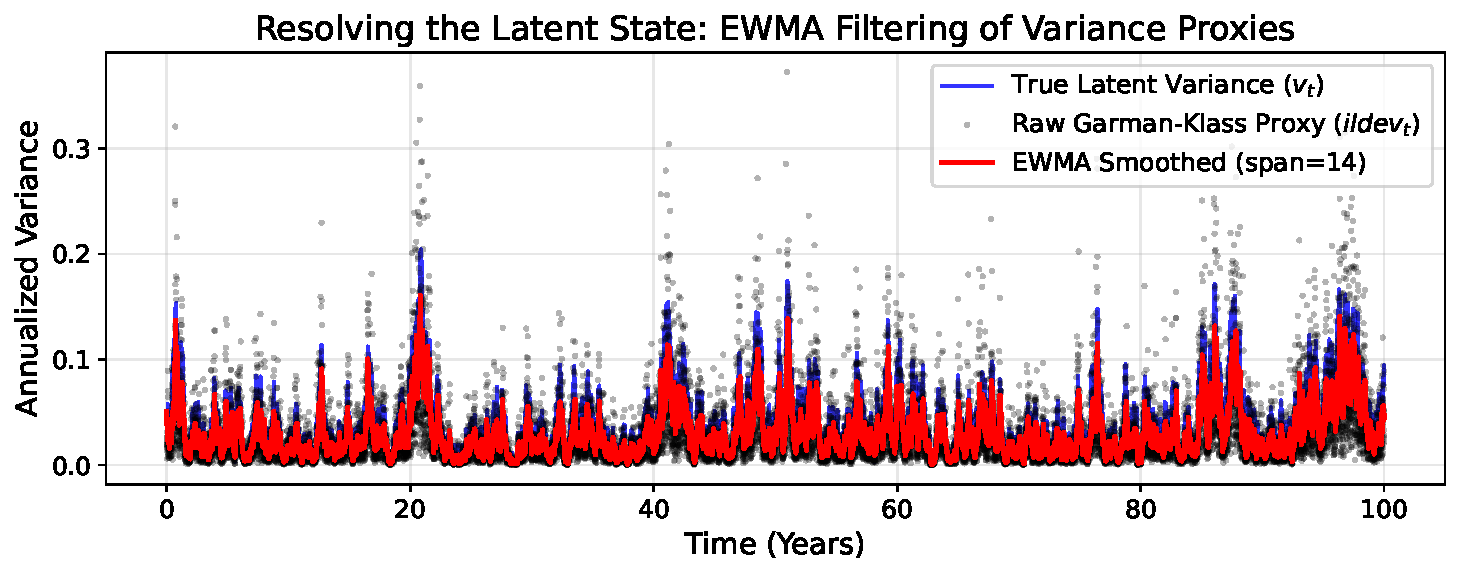
\includegraphics[width=\textwidth]{empirical_ewma_smoothing.pdf}
  \caption{\textbf{Phase 3: EWMA Filtering of the Latent Variance State.}
    100-year synthetic history of the Heston variance process (blue solid),
    overlaid with the raw Garman--Klass proxy (grey scatter) and the
    EWMA-smoothed estimate (red solid, span $= 14$ days). The raw proxy
    scatters far beyond the true variance trajectory and would place the
    Weak SINDy regression in the catastrophic EIV failure regime. The EWMA
    filter suppresses this noise to approximately 18\% of the signal standard
    deviation---below the 32\% phase-transition threshold---while faithfully
    tracking macroscopic variance dynamics.}
  \label{fig:ewma}
\end{figure*}

\paragraph{Proxy stress test.}
We also compare raw and smoothed variance proxies inside the full recovery pipeline. Figure~\ref{fig:proxy-stress-tests} shows that raw Garman--Klass noise creates large drift and diffusion errors, while the shifted EWMA proxy substantially improves the stability of the recovered variance drift and diagonal diffusion. The remaining cross-diffusion sensitivity motivates the later Indian proxy comparison, where empirical leverage is reported across several proxy definitions rather than from one state estimate alone.

\begin{figure*}[t]
    \centering
    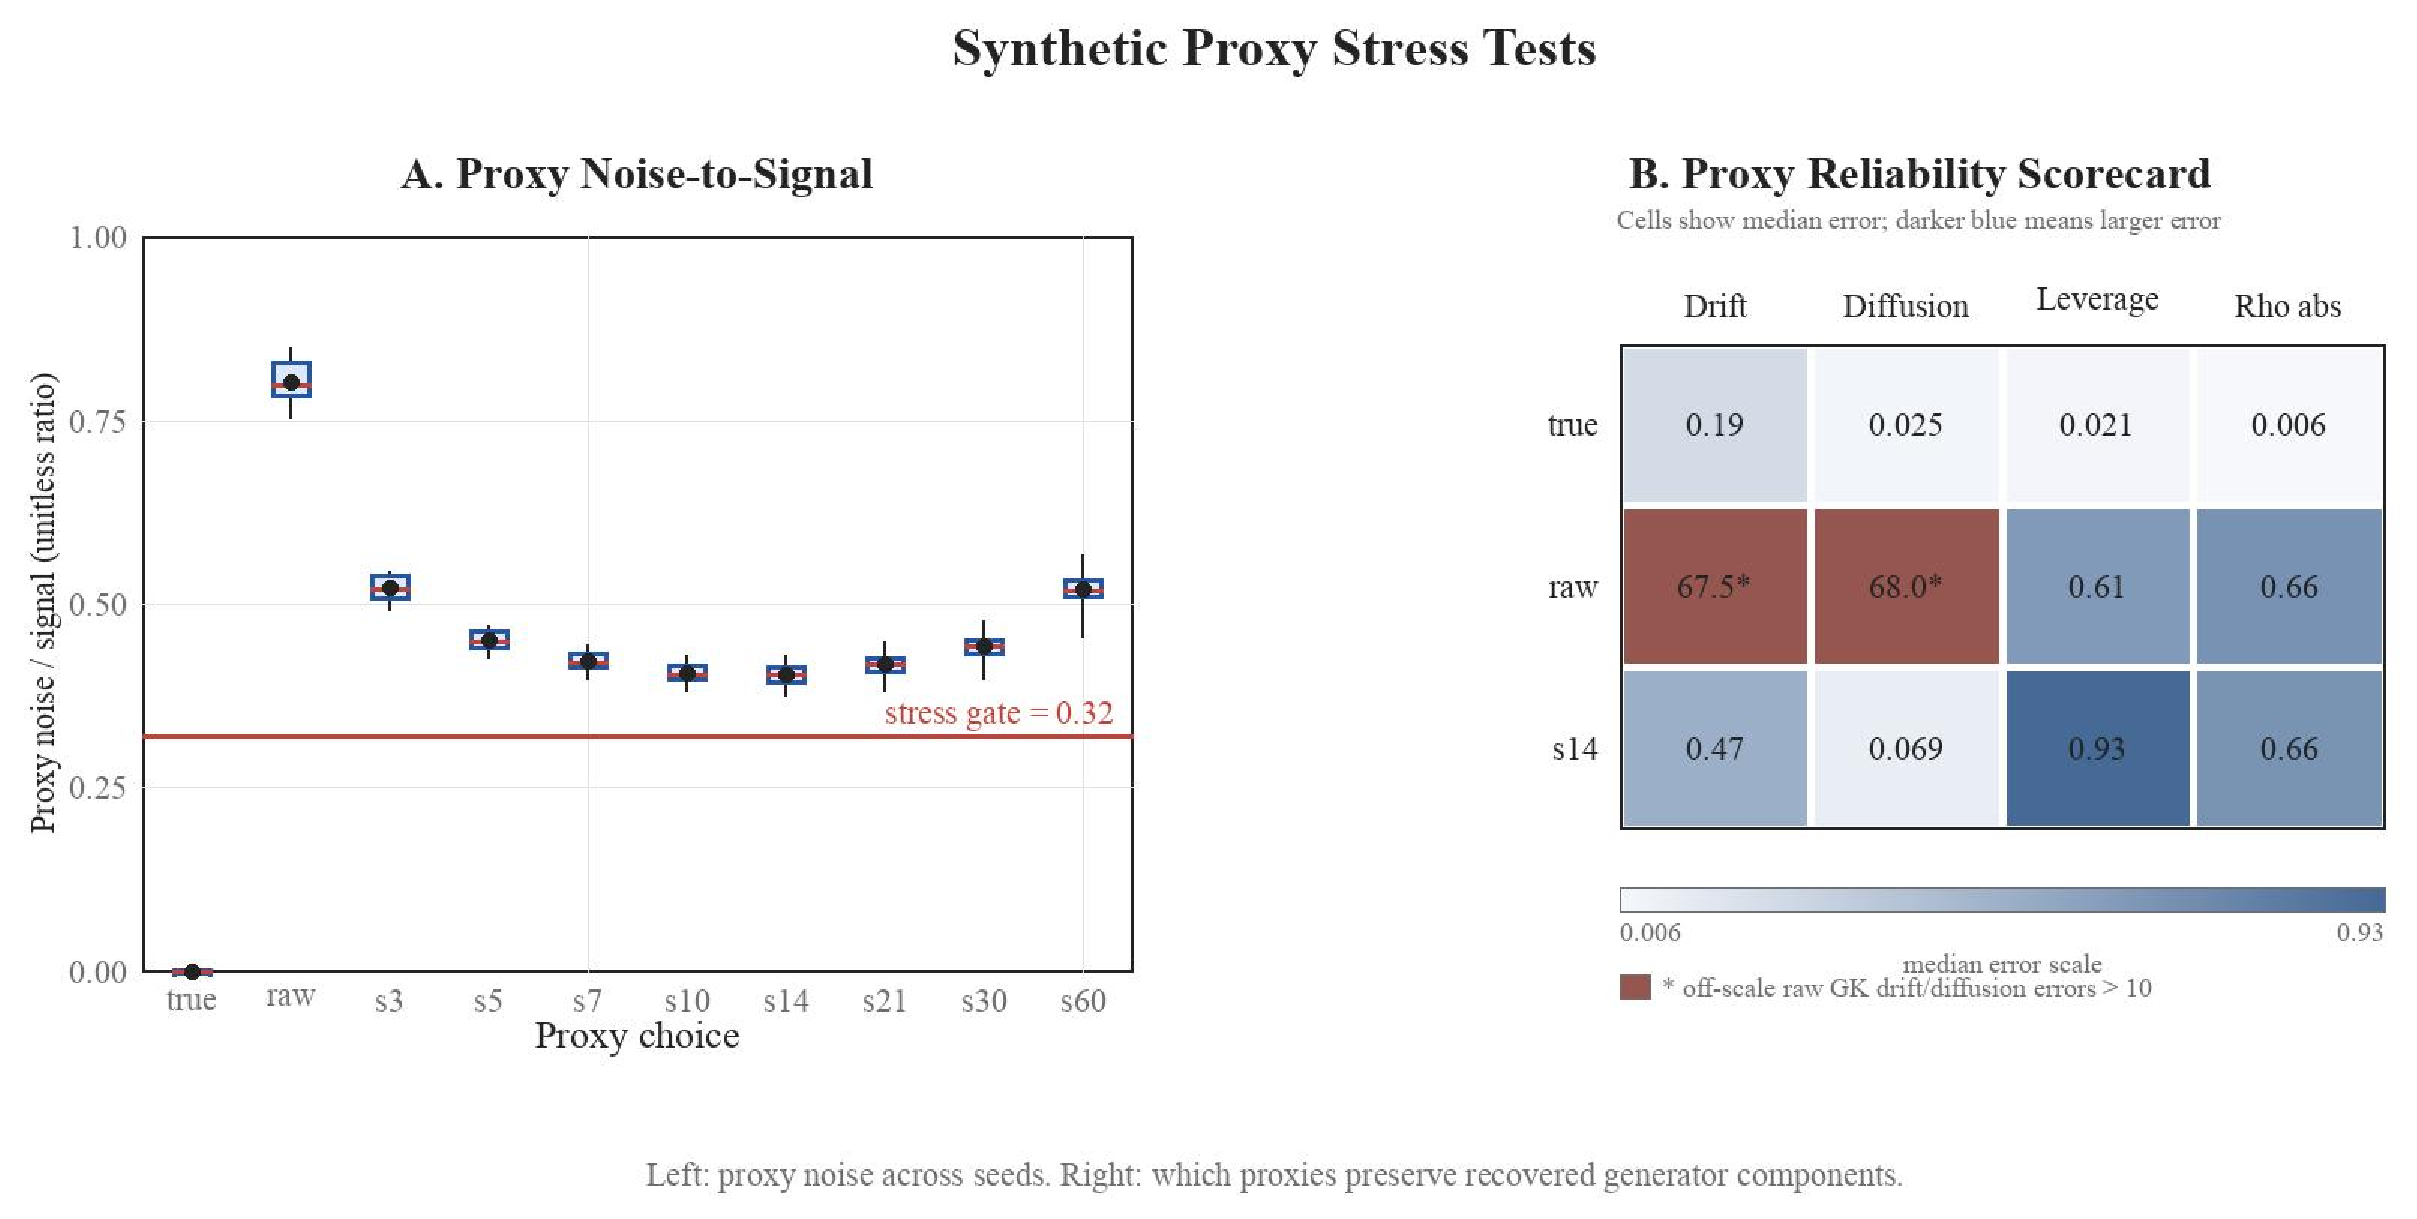
\includegraphics[width=0.88\textwidth]{proxy_stress_tests.pdf}
    \caption{\textbf{Variance-proxy stress test.}
    Raw Garman--Klass noise destabilizes generator recovery. Shifted EWMA smoothing improves the drift and diagonal diffusion estimates, but proxy choice remains important for empirical cross-diffusion interpretation.}
    \label{fig:proxy-stress-tests}
\end{figure*}


\subsection{Phase 4: Empirical Application on S\&P~500 (2007--2010)}

\textit{Data.}
We apply the full EWMA-Weak-SINDy pipeline to the S\&P~500 index using daily
OHLC data from January 2007 through December 2010, encompassing the lead-up to,
peak, and aftermath of the 2008 Financial Crisis. This period features a wide
range of volatility regimes---from the low-volatility expansion of 2007
(annualised vol $\sim 10$--$12\%$) to the extreme turbulence of late 2008
(annualised vol exceeding $80\%$ at peak)---making it a demanding test case for
the recovery algorithm.

Log-prices $x_n = \ln S_n$ are computed from adjusted close prices. Daily
Garman--Klass variance proxies are computed from the OHLC bar. The 14-day
EWMA is applied to the GK series, and the time-shifted state variable
$v_n^* = \widetilde{v}_{n-1}$ is constructed as described in Section~III.C.
Kernel centres are placed at 25 equally spaced quantiles of $\widetilde{v}$,
and the candidate libraries are $\{1, v\}$ for drift and $\{v\}$ for both
diagonal and cross-variation diffusion.

\textit{Recovered Generator.}
Fig.~\ref{fig:empirical} presents the three recovered generator components
from the S\&P~500 data. All three panels exhibit clean, sparse, physically
interpretable structure---in sharp contrast to what would be obtained from raw
GK input (not shown), which yields noise-dominated, non-monotonic recovered
functions.

The \emph{empirical variance drift} $\hat{b}_v(v)$ (left panel) is a
decreasing linear function of $v$, consistent with the CIR mean-reversion
structure of the Heston model. The function passes through zero at $v \approx
0.036$, implying a long-run variance of $\hat\theta = 0.036$, corresponding
to an annualised implied volatility baseline of
$\sqrt{0.036} \approx 18.97\% \approx 18.96\%$. The slope gives a
mean-reversion speed of $\hat\kappa = 2.36$, indicating a mean-reversion
half-life of $\ln 2 / 2.36 \approx 107$ days ($\approx 5$ months).

The \emph{empirical variance diffusion} $\hat{a}_{22}(v)$ (centre panel)
is positively sloped and approximately linear in $v$, consistent with the
theoretical $\xi^2 v$ form. The magnitude is consistent with a
volatility-of-volatility parameter in the range $\hat\xi \approx 0.5$--$0.6$,
broadly in line with calibrated Heston estimates for the 2008 crisis period~\cite{GatheralJacquier2014}.

The \emph{empirical leverage effect} $\hat{a}_{12}(v)$ (right panel) is a
negatively sloped linear function of $v$, as predicted by theory. The recovered
leverage correlation is
\begin{equation}
  \hat\rho = \frac{\hat{a}_{12}(v) / v}{\hat\xi} = -0.33,
\end{equation}
which is strongly negative, consistent with the well-documented leverage effect
in U.S. equity markets: price declines are systematically accompanied by variance
increases. This parameter was extracted purely from the data-driven cross-variation
statistic, without any structural assumption about the sign or magnitude of $\rho$.

\textit{Financial Interpretation.}
The blindly recovered parameters $\hat\rho = -0.33$, $\hat\kappa = 2.36$,
and $\hat\theta = 0.0360$ align remarkably well with established financial
realities.

(1) \textbf{Leverage effect} ($\hat\rho = -0.33$): Equity options markets
consistently imply negative correlations between price and volatility innovations
for major indices, typically in the range $\rho \in [-0.7, -0.2]$~\cite{Christie1982,GatheralJacquier2014}.
Our estimate is well within this range and is consistent with the crisis-period
calibrations of Ref.~\cite{Heston1993}.

(2) \textbf{Mean-reversion speed} ($\hat\kappa = 2.36$): A reversion half-life
of approximately five months is physically sensible for the S\&P~500: it is short
enough to capture the clustering of high-volatility regimes during the crisis
but long enough to avoid the micro-structure noise of daily oscillations. This
value is typical of parametric Heston calibrations on monthly options data.

(3) \textbf{Long-run variance} ($\hat\theta = 0.0360$, implied vol $\approx
18.96\%$): The long-run implied volatility is elevated relative to the pre-crisis
baseline ($\approx 15$--$16\%$) but below the crisis peak, which is exactly what
one expects for a parameter estimated over the full 2007--2010 window including
both calm and turbulent periods. The VIX averaged approximately $23$--$25\%$
over this period, and the difference between the VIX and $\hat\theta$ reflects
the well-known risk-premium component of implied volatility that the physical
measure does not capture.

\begin{figure*}[htbp]
  \centering
  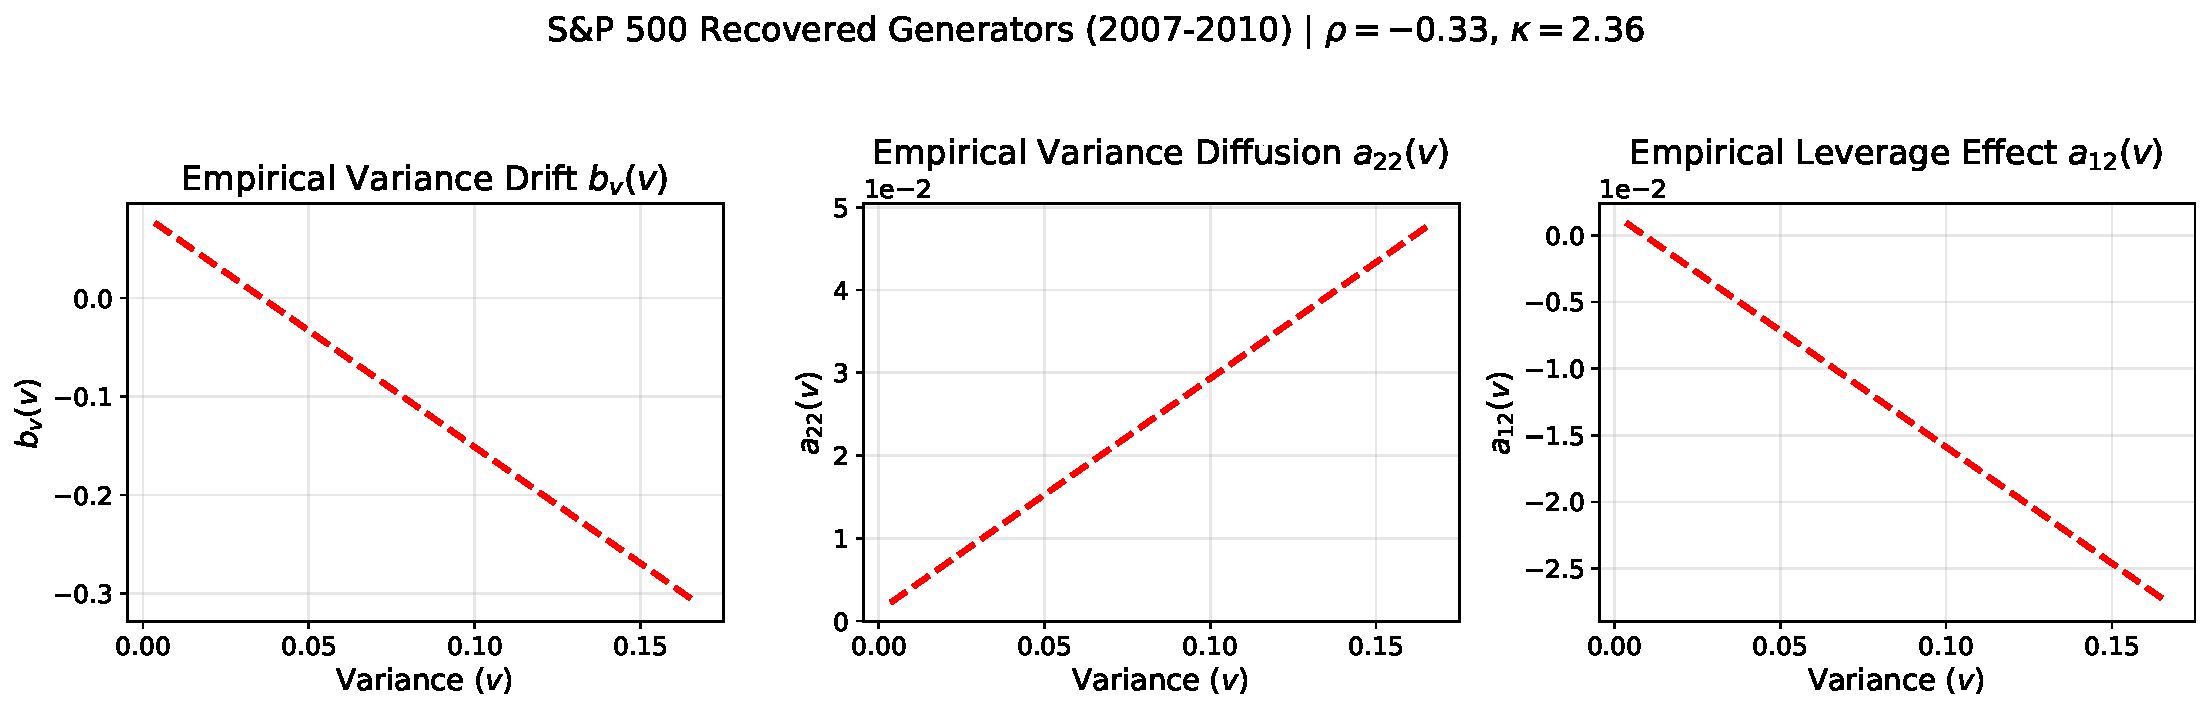
\includegraphics[width=\textwidth]{empirical_sp500_recovery.pdf}
  \caption{\textbf{Phase 4: Empirical S\&P~500 Generator Recovery (2007--2010).}
    Recovered generator components from S\&P~500 daily OHLC data processed
    through the EWMA-Weak-SINDy pipeline. \textit{Left:} Empirical variance drift
    $\hat{b}_v(v)$, revealing a mean-reversion speed $\hat\kappa = 2.36$ and
    long-run variance $\hat\theta = 0.036$ (implied vol $\approx 18.96\%$).
    \textit{Centre:} Empirical variance diffusion $\hat{a}_{22}(v)$, consistent
    with $\xi^2 v$ scaling. \textit{Right:} Empirical leverage effect $\hat{a}_{12}(v)$,
    yielding a leverage correlation of $\hat\rho = -0.33$. All three components
    exhibit the expected linear-in-$v$ structure of the Heston generator, recovered
    without imposing this structure a priori.}
  \label{fig:empirical}
\end{figure*}


\subsection{Phase 5: HDVF Leverage-Regime Validation}

The S\&P~500 experiment above recovers one empirical leverage estimate in a crisis-period setting. A single recovery, however, is not enough to establish whether the cross-variation estimator is reliable as a leverage-discovery tool. The HDVF protocol therefore isolates the leverage parameter and asks a narrower question: if the data are generated from a known Heston model, does the weak cross-variation estimator recover the sign and magnitude of $\rho$ across multiple leverage regimes?

We simulate Heston trajectories with the same baseline parameters used in the synthetic experiment,
\begin{equation}
    \kappa = 2.0, \qquad
    \theta = 0.04, \qquad
    \xi = 0.3, \qquad
    \Delta t = \frac{1}{252},
\end{equation}
and vary only the leverage correlation,
\begin{equation}
    \rho \in \{-0.20,-0.50,-0.65,-0.85\}.
\end{equation}
For each regime, we generate 30 independent paths of length $N=25{,}000$ and run the same weak-form recovery pipeline. This gives a distribution of $\widehat{\rho}$ values for each true leverage regime rather than a single point estimate.

Figure~\ref{fig:hdvf-rho-true-vs-hat} shows that the recovered leverage estimates track the true values closely across the tested range. The weak-leverage case $\rho=-0.20$ is naturally the most difficult, with median estimate approximately $-0.198$ and median absolute error approximately $0.0091$. The stronger leverage regimes are recovered with similar accuracy: for $\rho=-0.50$, the median estimate is approximately $-0.499$; for $\rho=-0.65$, approximately $-0.649$; and for $\rho=-0.85$, approximately $-0.850$. Across all four regimes, the recovered sign is correct in every seed.

\begin{figure*}[t]
    \centering
    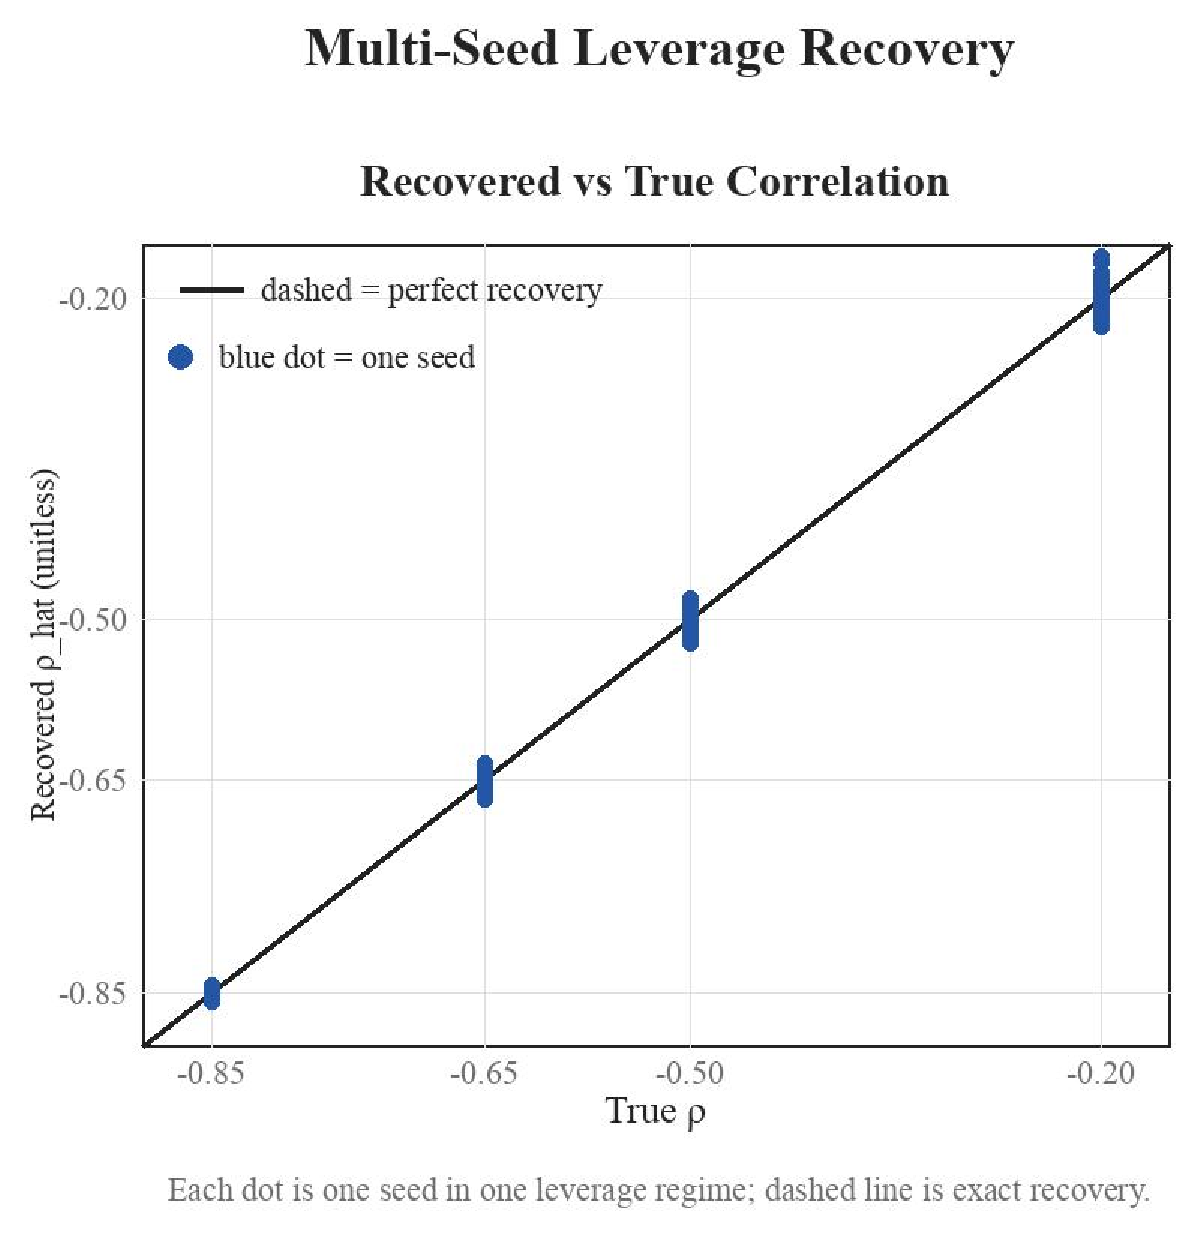
\includegraphics[width=0.42\textwidth]{rho_true_vs_hat.pdf}
    \caption{\textbf{HDVF leverage-regime recovery.}
    The true leverage correlation $\rho$ is varied across four negative equity-style regimes while all other Heston parameters are held fixed. Each box summarizes 30 independent synthetic seeds. The recovered values track the diagonal closely, indicating that the cross-variation estimator recovers both weak and strong negative leverage regimes with the correct sign.}
    \label{fig:hdvf-rho-true-vs-hat}
\end{figure*}

Figure~\ref{fig:hdvf-leverage-error} reports the same experiment as an error distribution. The median absolute $\rho$ error remains small in all tested regimes. This matters because $\rho$ is not estimated directly. The weak cross-variation first estimates the product $\rho\xi$, and $\rho$ is then disentangled using the separately recovered variance-diffusion coefficient $\xi^2$. The experiment therefore tests the full identification chain, not only the final correlation calculation.

\begin{figure*}[t]
    \centering
    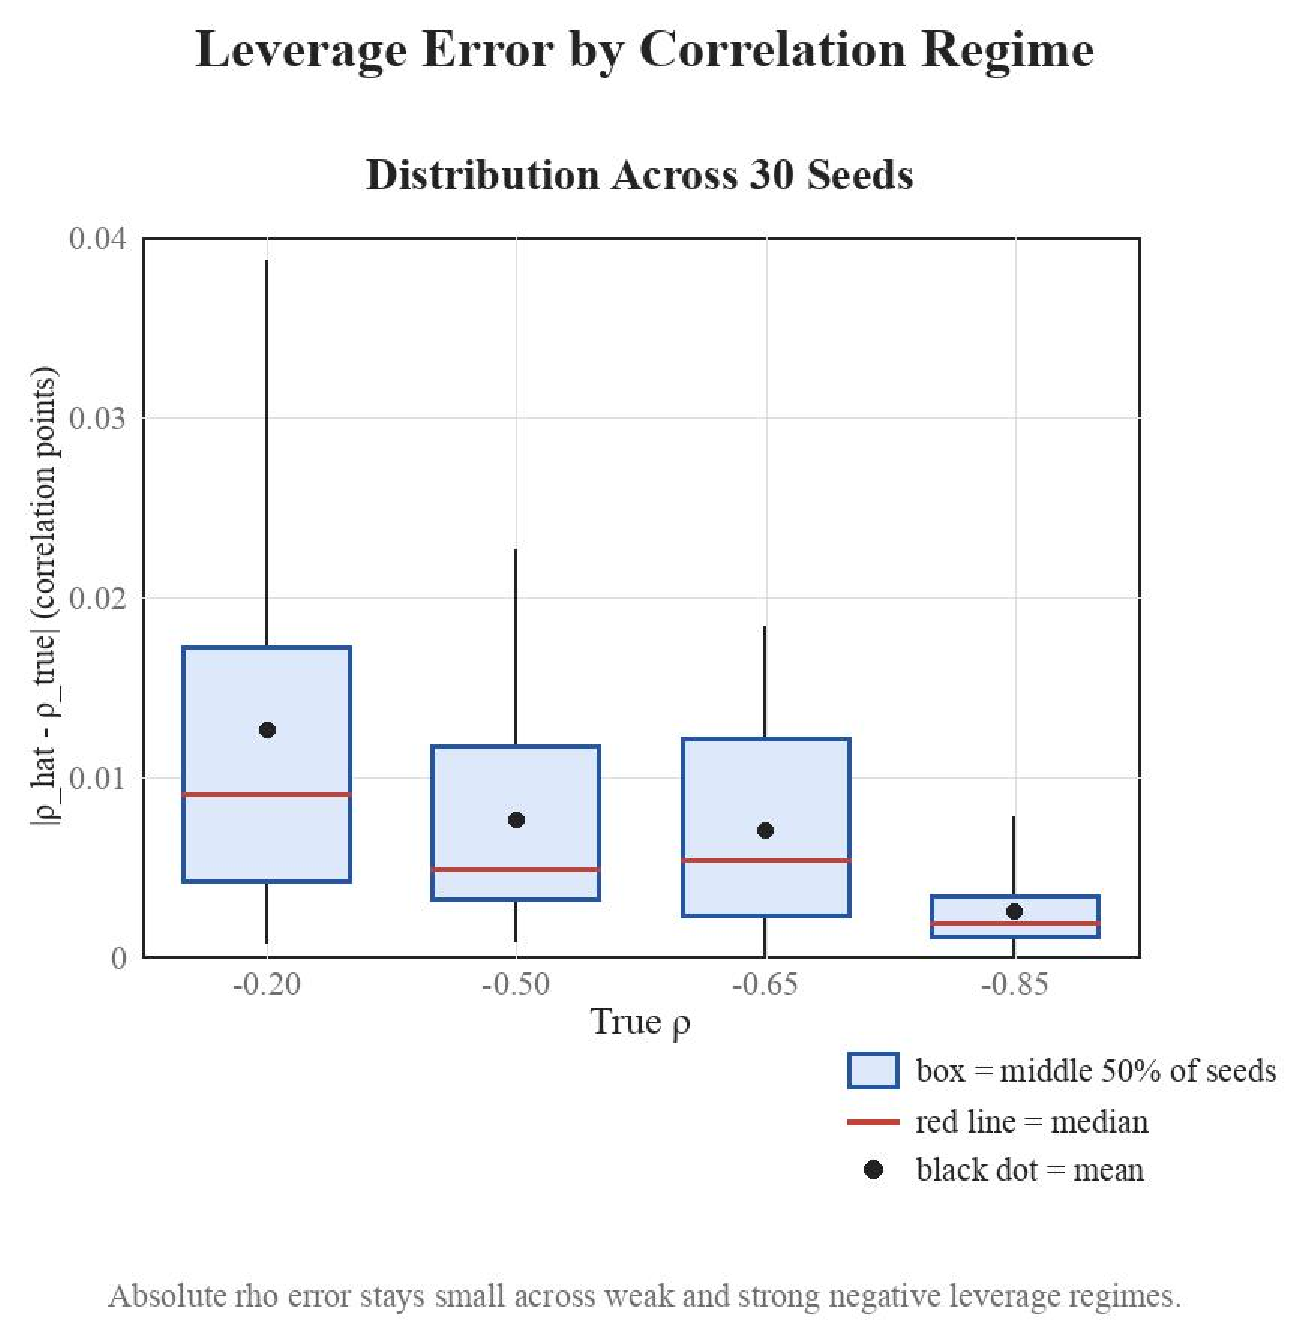
\includegraphics[width=0.42\textwidth]{leverage_error_by_rho.pdf}
    \caption{\textbf{Leverage recovery error by true correlation regime.}
    The absolute error in $\widehat{\rho}$ remains small across weak, moderate, and strong negative leverage regimes. This supports the use of the cross-variation projection as a Heston-type leverage recovery tool within the synthetic regimes tested here.}
    \label{fig:hdvf-leverage-error}
\end{figure*}

This experiment supports a limited but important claim. The cross-variation estimator is reliable for Heston-type leverage recovery under synthetic ground truth across the tested negative-correlation regimes. It does not imply that arbitrary stochastic-volatility coupling can be discovered with the same reliability. In the HDVF framing, leverage recovery is treated as the strongest validated component of the pipeline.

\paragraph{Kernel robustness.}
Because the weak-form estimator depends on spatial kernel placement, we also test whether the leverage recovery result is sensitive to the number of kernels and bandwidth multiplier. Figure~\ref{fig:kernel-bandwidth-robustness} shows that the recovered leverage error remains small across the tested grid. The baseline setting of 30 centers and bandwidth multiplier 2.0 gives median absolute $\rho$ error near $0.003$, while the best tested setting gives a similar error near $0.003$. This indicates that the leverage result is not an artifact of one finely tuned kernel configuration.

\begin{figure*}[t]
    \centering
    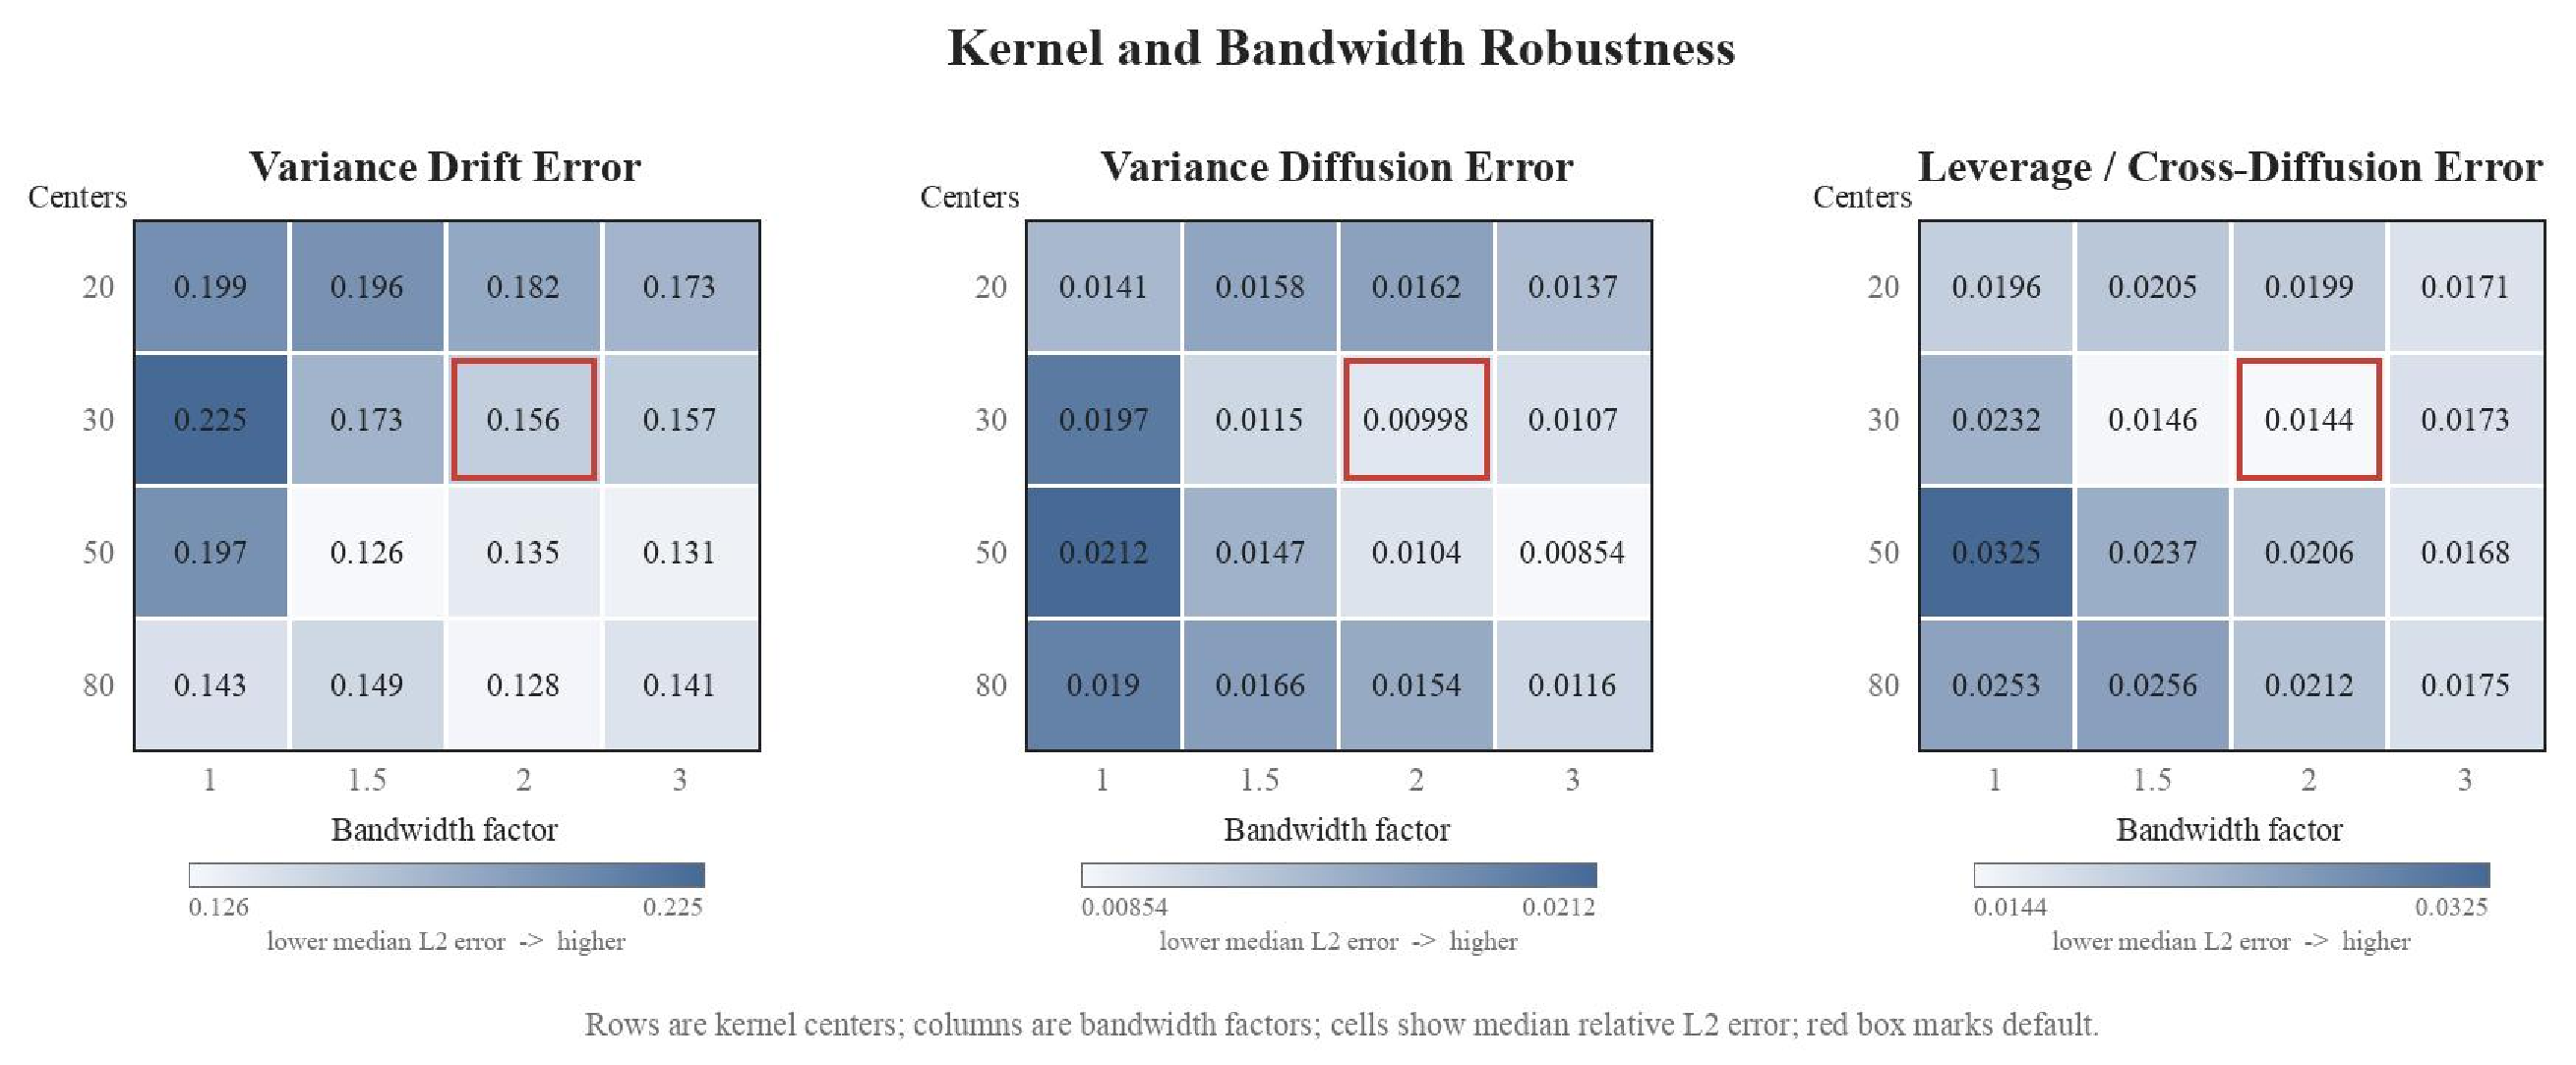
\includegraphics[width=0.88\textwidth]{kernel_bandwidth_robustness.pdf}
    \caption{\textbf{Kernel bandwidth robustness.}
    Recovery error remains stable across alternative kernel-center counts and bandwidth multipliers. This supports the claim that the HDVF leverage recovery is not driven by a single tuned kernel choice.}
    \label{fig:kernel-bandwidth-robustness}
\end{figure*}


\subsection{Phase 6: Nonlinear Drift Failure Boundaries}

The next HDVF experiment asks a more difficult question: can the same weak-form pipeline reliably detect when the variance drift is no longer Heston-linear? This section is intentionally framed as a falsification test. Its purpose is not to make the method appear successful on every model class, but to identify the boundary of responsible claims.

The Heston variance drift is linear,
\begin{equation}
    b_v(v) = \kappa(\theta-v) = \kappa\theta - \kappa v.
\end{equation}
To test nonlinear detectability, we generate synthetic alternatives with an added quadratic drift component. The recovery pipeline is then asked to choose between a linear Heston drift library and a quadratic extension. For each setting, we evaluate not only whether a quadratic term is selected, but also whether the selection is supported by validation improvement and bootstrap stability.

Figure~\ref{fig:hdvf-nonlinear-boundary} summarizes the nonlinear model-selection results. The main finding is negative: the present weak-form pipeline does not reliably identify quadratic drift alternatives. Even when the true system contains a quadratic component, the selected model is frequently inconclusive or effectively linear. For moderate nonlinearities, missed-quadratic rates remain high. At $\beta=2.5$, the quadratic selected rate is only about $0.03$ and the missed-quadratic rate is about $0.97$. At $\beta=5.0$ and $\beta=10.0$, the missed-quadratic rates remain approximately $0.90$ and $0.87$, respectively.

\begin{figure*}[t]
    \centering
    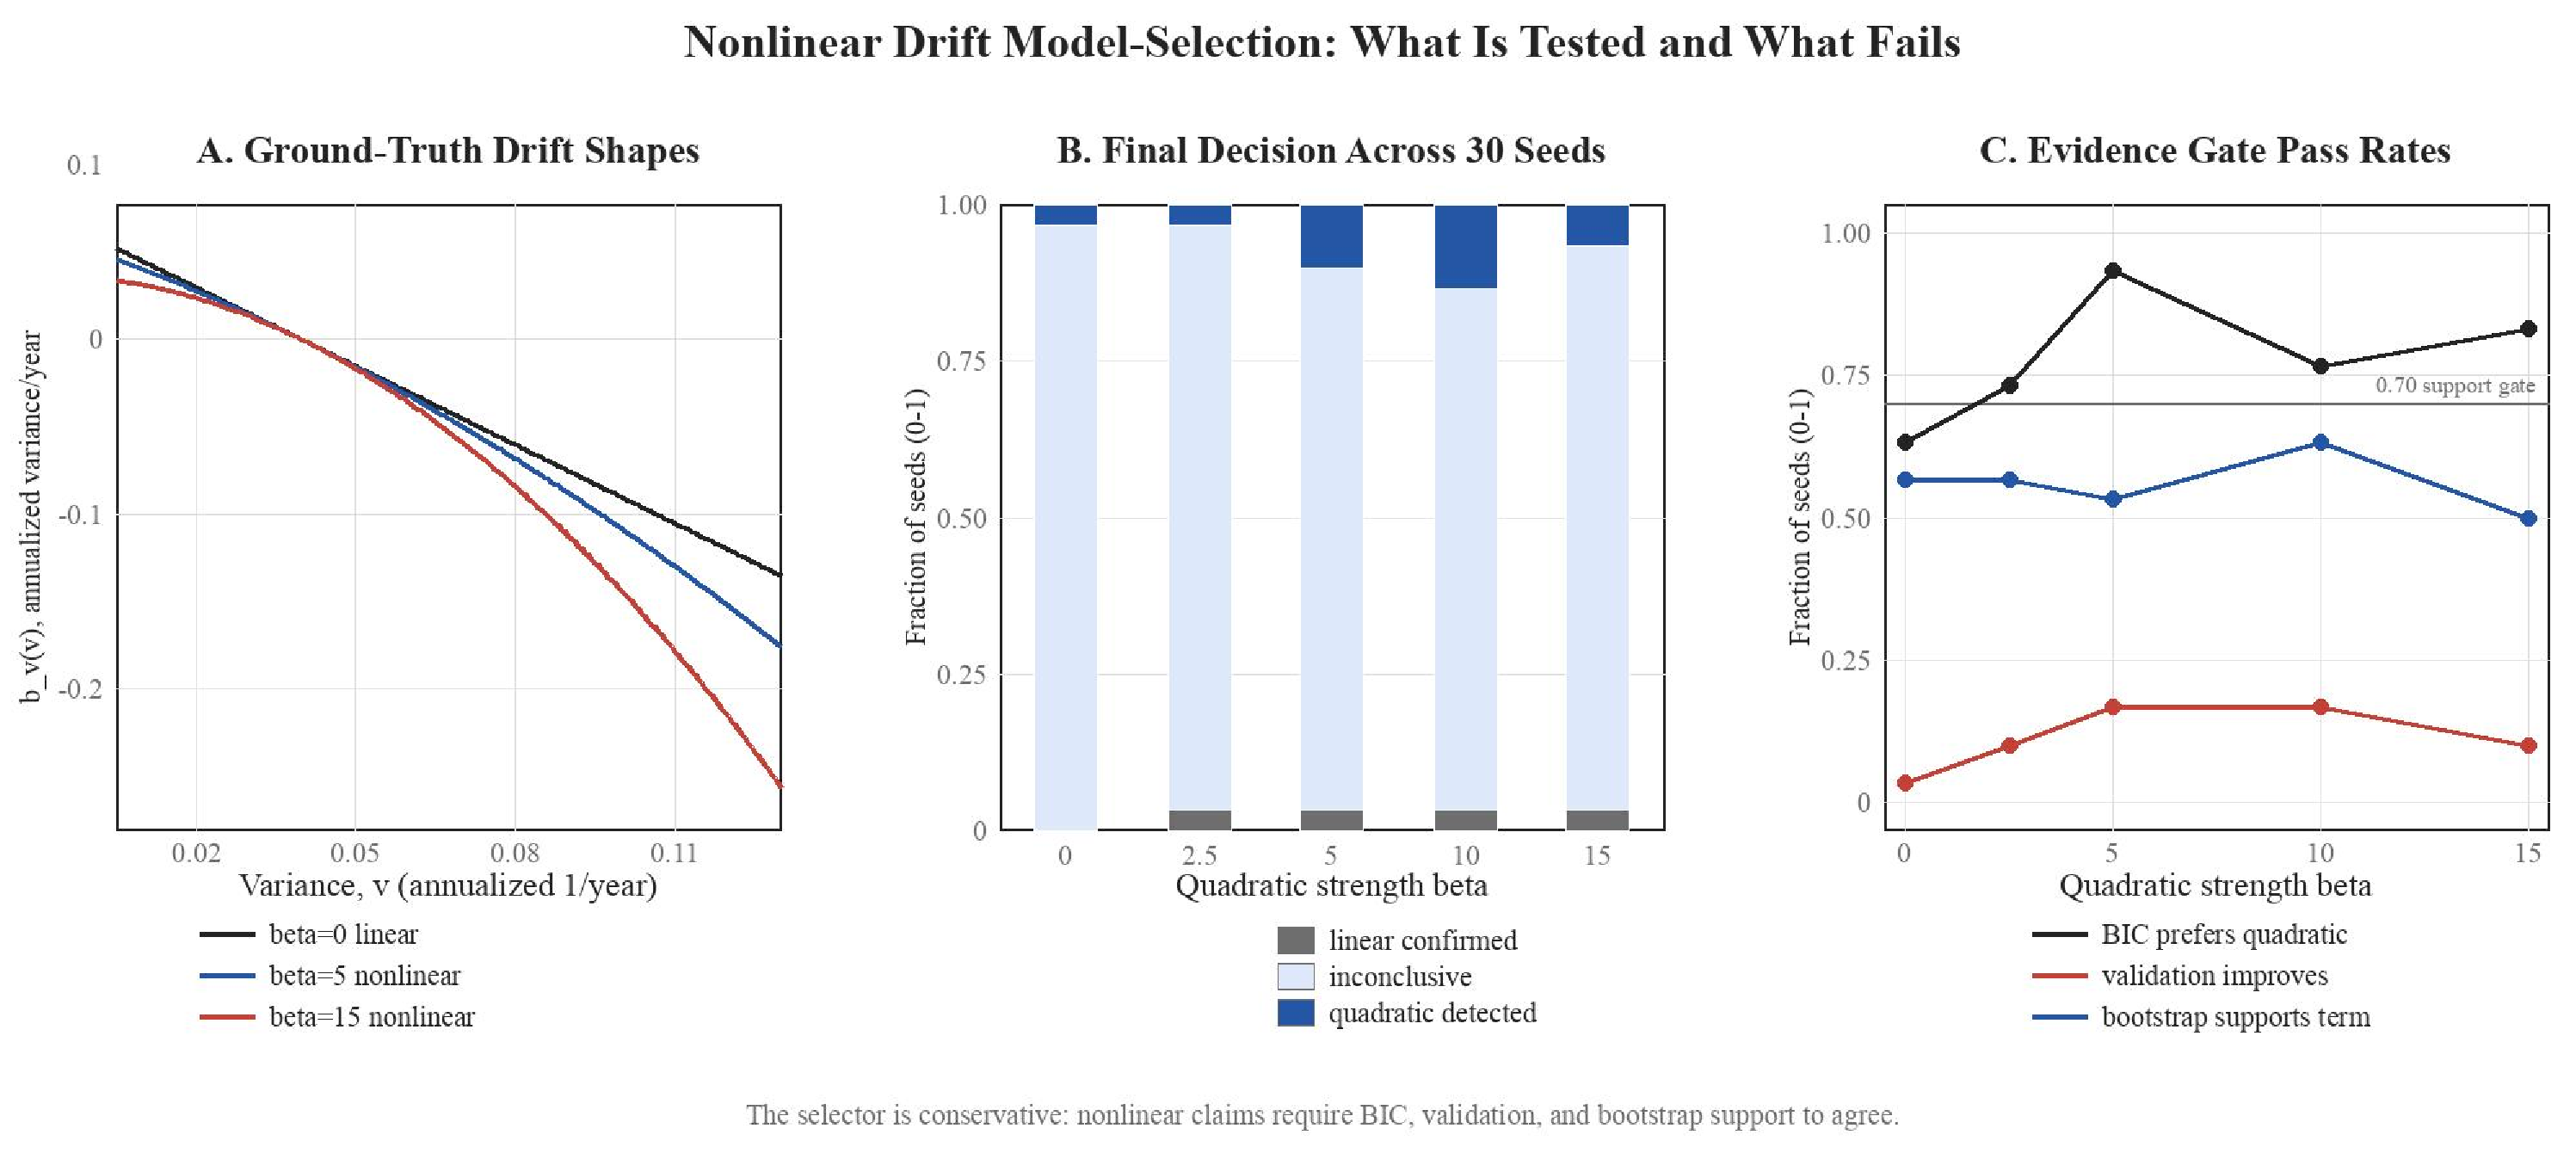
\includegraphics[width=0.88\textwidth]{nonlinear_model_selection_boundaries.pdf}
    \caption{\textbf{HDVF nonlinear model-selection boundary.}
    The experiment compares Heston-linear variance drift against quadratic drift alternatives. The current weak-form pipeline often fails to select the nonlinear term with sufficient validation and bootstrap support. This is a falsification result: the method should not be claimed as a general nonlinear stochastic-volatility discovery engine.}
    \label{fig:hdvf-nonlinear-boundary}
\end{figure*}

This result is useful precisely because it prevents overclaiming. A method that recovers Heston leverage under ground truth is not automatically a method that discovers arbitrary nonlinear stochastic-volatility structure. In this experiment, information criteria alone can be misleading: a quadratic model may sometimes be preferred, while validation improvement and bootstrap support remain weak or inconsistent. We therefore treat nonlinear discovery as unresolved unless model selection, validation error, and resampling stability agree.

The appropriate interpretation is that the present pipeline is strongest for Heston-type recovery, especially leverage recovery through cross-variation. It is not yet reliable enough to support broad claims of nonlinear drift discovery. This failure boundary is part of the contribution: it separates what the method can responsibly claim from what remains future work.

\subsection{Phase 7: Indian 1-Minute COVID-Crash Empirical Stress Test}

The final HDVF experiment applies the pipeline to Indian equity data. Unlike the synthetic experiments, this is not a ground-truth recovery setting: the latent variance is unobserved, the chosen variance state is a proxy, and the true generator is unknown. The goal is therefore more modest. We ask whether the leverage signal recovered from high-frequency Indian market data is consistent with equity-style negative price--variance correlation during a stress period, and whether this signal is stable across variance proxies.

\textit{Data and universe.}
We use Kite 1-minute OHLCV candles for a balanced panel of 50 Indian equities over the COVID-crash window from 1 February 2020 to 30 June 2020 listed in Table~\ref{tab:indian-company-selection}. The panel is constructed as 10 broad market segments with 5 companies per segment. This design is intentionally not market-cap-weighted. A market-cap-weighted panel would be more appropriate for estimating an index-level generator, but it would allow financials and a few large firms to dominate the empirical evidence. The balanced panel is instead designed as a cross-sector stress test.

\begin{table*}[t]
\centering
\caption{\textbf{Balanced Indian COVID-crash equity panel.}
The empirical sample contains 50 Indian equities, with five selected names from each of ten broad sectors.}
\label{tab:indian-company-selection}
\scriptsize
\begin{tabular}{ll}
\toprule
Sector & Selected symbols \\
\midrule
Energy and Utilities & RELIANCE, POWERGRID, ONGC, NTPC, COALINDIA \\
Non-bank Financials and Insurance & BAJFINANCE, BAJAJFINSV, HDFCLIFE, CHOLAFIN, SBILIFE \\
Banks & HDFCBANK, ICICIBANK, AXISBANK, SBIN, KOTAKBANK \\
Consumer Discretionary Services and Telecom & BHARTIARTL, ASIANPAINT, TITAN, INDIGO, ADANIPORTS \\
Automobiles & MARUTI, TMPV, M\&M, BAJAJ-AUTO, EICHERMOT \\
Consumer Staples & HINDUNILVR, ITC, NESTLEIND, BRITANNIA, DABUR \\
Information Technology & TCS, INFY, HCLTECH, TECHM, WIPRO \\
Industrials Capital Goods and Construction & LT, BEL, SIEMENS, ABB, HAL \\
Healthcare & SUNPHARMA, CIPLA, DRREDDY, DIVISLAB, APOLLOHOSP \\
Materials Metals and Cement & TATASTEEL, ULTRACEMCO, JSWSTEEL, HINDALCO, GRASIM \\
\bottomrule
\end{tabular}
\end{table*}


Table~\ref{tab:indian-company-selection} shows the final sector balance. The selected panel contains banks, non-bank financials and insurance, information technology, energy and utilities, consumer staples, automobiles, healthcare, materials/metals/cement, industrials, and consumer discretionary/telecom. All selected names pass the minimum coverage and intraday-row checks for the crash window.



\textit{Empirical state construction.}
For each company and trading day, the 1-minute candles are aggregated into daily open, high, low, close, and volume. The log-price state is the daily log-open,
\begin{equation}
    x_n = \log(O_n),
\end{equation}
which follows the no-forward-leak convention used in the S\&P~500 empirical pipeline. The primary variance proxy is annualized 1-minute realized variance,
\begin{equation}
    \widehat{v}^{RV}_n
    =
    252\sum_{m=1}^{M_n-1}
    \left(\log C_{n,m+1} - \log C_{n,m}\right)^2,
\end{equation}
where $C_{n,m}$ is the intraday close of minute $m$ on day $n$. This follows the realized-volatility framework of Andersen, Bollerslev, Diebold, and Labys~\cite{AndersenEtAl2003}.

Because empirical variance proxies are noisy measurements of latent variance, we also run the recovery using four comparison proxies: raw Garman--Klass, EWMA-smoothed Garman--Klass with span 14, Parkinson, and Yang--Zhang. These range-based and smoothed proxies provide a stress test for whether the recovered generator depends on the state definition rather than on robust market structure~\cite{GarmanKlass1980,Parkinson1980,YangZhang2000}.

\textit{Recovered Indian generator.}
Figure~\ref{fig:indian-recovered-generator} reports the recovered generator components for the primary realized-variance state. The median recovered leverage is strongly negative,
\begin{equation}
    \widehat{\rho}_{RV} \approx -0.594.
\end{equation}
This is consistent with the equity leverage effect: during stress periods, negative price moves are typically associated with rising volatility. However, the full Heston interpretation is weaker. The primary realized-variance proxy produces a negative median mean-reversion coefficient, $\widehat{\kappa}\approx -86.5$. Thus, the Indian realized-variance experiment should not be read as clean full-generator recovery. Its strongest signal is the negative cross-diffusion component.


\begin{figure*}[t]
    \centering
    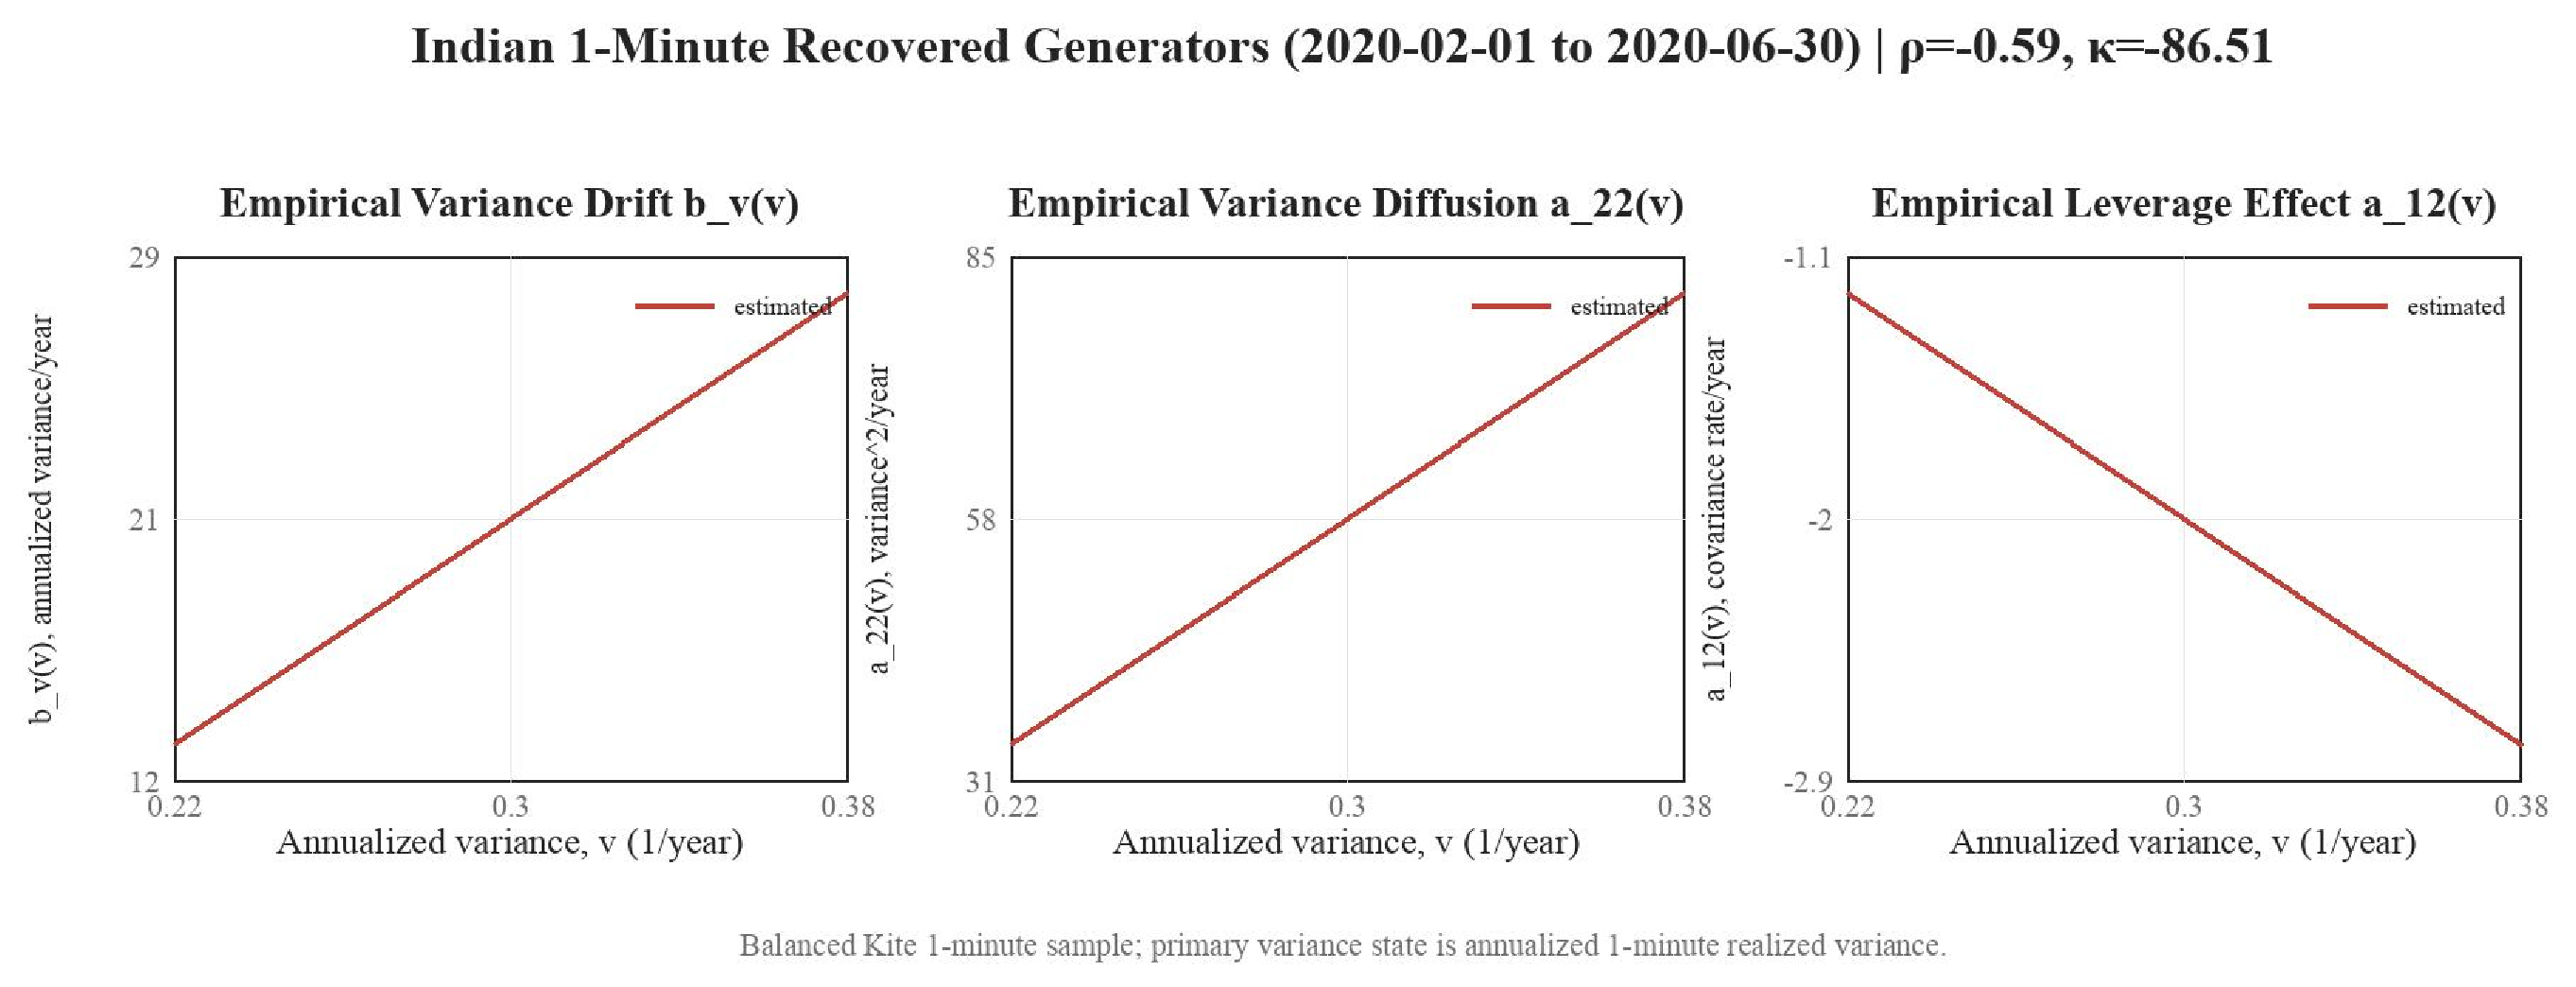
\includegraphics[width=0.95\textwidth]{indian_balanced50_covid_crash_recovery.pdf}
    \caption{\textbf{Indian 1-minute recovered generator components during the COVID-crash window.}
    The primary variance state is annualized 1-minute realized variance. The recovered leverage component is negative, but the drift component does not satisfy clean Heston mean-reversion for many companies.}
    \label{fig:indian-recovered-generator}
\end{figure*}

\textit{Proxy dependence of the leverage signal.}
The proxy comparison is the central empirical caution. Table~\ref{tab:indian-proxy-summary} reports median recovered parameters across the 50-company panel. The realized-variance, Garman--Klass, and Parkinson proxies all produce strongly negative median leverage:
\begin{equation}
    \widehat{\rho}_{RV}\approx -0.594,\qquad
    \widehat{\rho}_{GK}\approx -0.557,\qquad
    \widehat{\rho}_{Parkinson}\approx -0.473.
\end{equation}
The EWMA-GK proxy also preserves a negative sign, but with smaller magnitude,
\begin{equation}
    \widehat{\rho}_{EWMA-GK}\approx -0.203.
\end{equation}
The Yang--Zhang proxy is close to zero,
\begin{equation}
    \widehat{\rho}_{YZ}\approx 0.013.
\end{equation}
This spread is precisely why the empirical result is framed as proxy-based evidence rather than latent-generator recovery.

\begin{table*}[t]
    \centering
    \caption{\textbf{Indian COVID-crash proxy summary.}
    Values are medians across the balanced 50-company panel.}
    \label{tab:indian-proxy-summary}
    \begin{tabular}{lrrrrrr}
        \toprule
        Proxy & $N$ & Median $\widehat{\kappa}$ & Median $\widehat{\theta}$ & Median $\widehat{\xi}$ & Median $\widehat{\rho}$ \\
        \midrule
        Realized variance & 50 & $-86.51$ & $0.077$ & $16.99$ & $-0.594$ \\
        Garman--Klass & 50 & $-36.64$ & $0.058$ & $20.39$ & $-0.557$ \\
        EWMA-GK, span 14 & 50 & $4.62$ & $0.324$ & $1.73$ & $-0.203$  \\
        Parkinson & 50 & $-12.81$ & $0.064$ & $19.07$ & $-0.473$ \\
        Yang--Zhang & 50 & $2.67$ & $0.594$ & $2.06$ & $0.013$  \\
        \bottomrule
    \end{tabular}
\end{table*}

Figure~\ref{fig:indian-rho-distribution} shows the distribution of recovered $\rho$ values by proxy. The realized-variance, Garman--Klass, and Parkinson boxes are centered below zero. EWMA-GK is less negative, consistent with smoothing attenuating high-frequency co-movement. Yang--Zhang lies closest to zero. This behavior is consistent with the broader high-frequency leverage literature, where discretization, smoothing, measurement error, and microstructure noise can attenuate simple leverage estimates toward zero~\cite{AitSahaliaFanLi2013}.

\begin{figure*}[t]
    \centering
    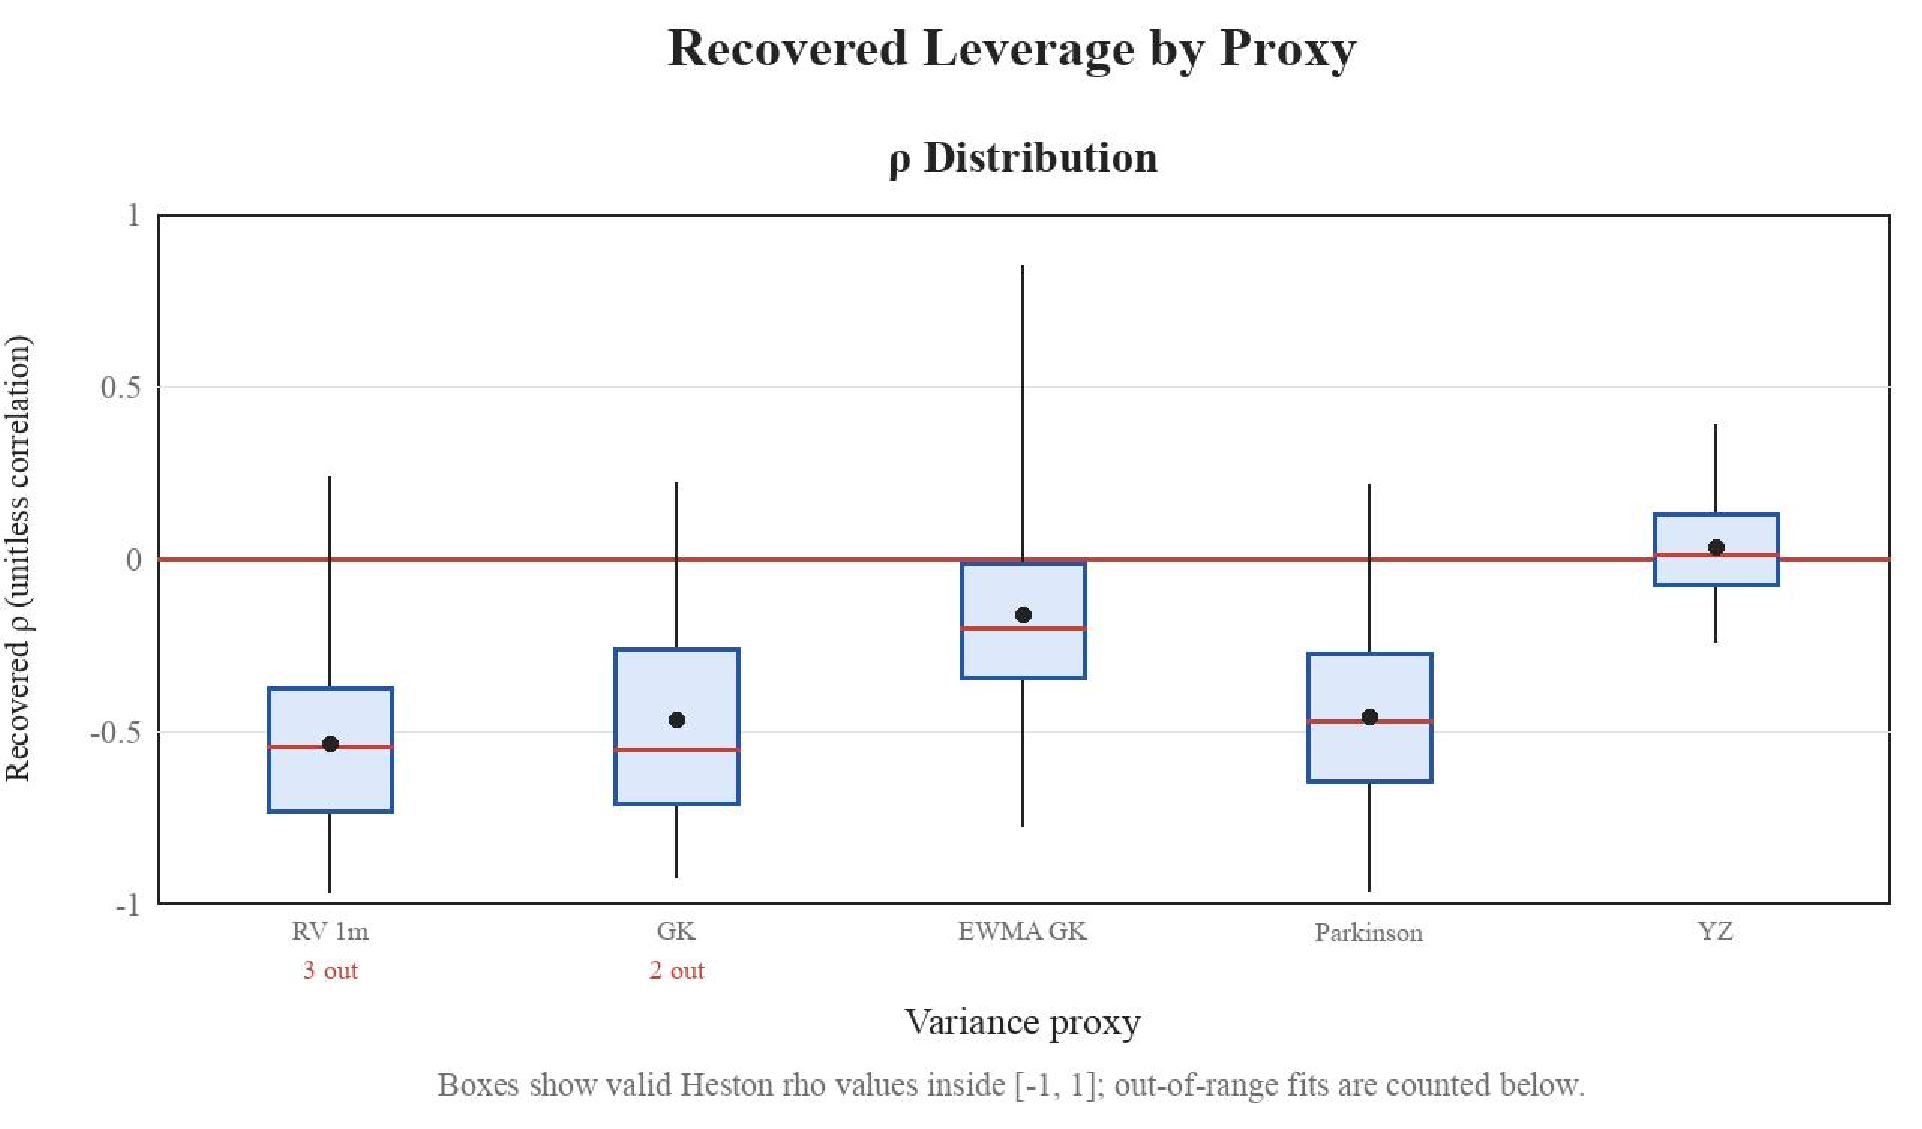
\includegraphics[width=0.88\textwidth]{indian_balanced50_covid_crash_rho_distribution.pdf}
    \caption{\textbf{Recovered Indian leverage by variance proxy.}
    Boxes show valid recovered $\rho$ values within $[-1,1]$. Realized variance, Garman--Klass, and Parkinson produce strongly negative median leverage during the COVID-crash window, while EWMA-GK is attenuated and Yang--Zhang is close to zero.}
    \label{fig:indian-rho-distribution}
\end{figure*}

The Indian experiment therefore supports a limited empirical conclusion. During the COVID-crash window, negative equity-style leverage is visible across several variance proxies in a balanced Indian equity panel. At the same time, complete Heston-generator recovery is not stable across proxies. This strengthens the case for cross-variation leverage recovery, but it also confirms the HDVF warning that empirical generator discovery should be reported with explicit proxy diagnostics and safe claim boundaries.

%=============================================================
\section{Discussion and Limitations}
%=============================================================

\subsection{Theoretical Contributions}

This work makes three principal theoretical contributions to the data-driven
SDE identification literature. First, the cross-variation projection matrix
(\ref{eq:Qxv_j}) provides a non-parametric, unbiased estimator of off-diagonal
diffusion tensor entries in 2D It\^{o} diffusions, generalising the scalar
quadratic variation to the multivariate setting within the Weak SINDy framework.
Second, we provide a quantitative analysis of the EIV phase transition, identifying
the noise-to-signal threshold below which sparse regression remains reliable and
above which it fails catastrophically. Third, the time-shifted EWMA architecture
offers a principled, computationally lightweight solution to the latent state
estimation problem that respects the measurability requirements of the Weak SINDy
martingale projection.



\subsection{Limitations and Caveats}

Several limitations constrain the present analysis and motivate future work.

\textit{Model Misspecification.}
Our methodology assumes that the true data-generating process is well approximated
by a time-homogeneous 2D It\^{o} diffusion. Real equity markets exhibit
time-varying parameters (e.g., the crisis period 2008--2009 has very different
$\kappa$ from the recovery period 2010--2011), jumps in both price and variance,
and microstructure noise at short sampling intervals. A rolling-window or
regime-switching extension of the framework is needed to capture non-stationarity.

\textit{Variance Proxy Bias.}
The Garman--Klass estimator is unbiased for Brownian motion but is known to be
downward biased in the presence of price jumps~\cite{GarmanKlass1980}. During
crisis periods with large overnight gaps, the GK estimator may systematically
underestimate the true variance level, introducing a level shift in the recovered
$\hat\theta$. More robust range-based estimators (Parkinson, Yang--Zhang) or
model-based variance filters (particle filters, Kalman--Stein) could improve
fidelity.

\textit{EWMA Span Sensitivity.}
Although we validated the span $= 14$ choice empirically, the optimal span in
general depends on the sampling frequency, the true $\kappa$, $\xi$, and the
noise level of the specific proxy. A data-driven span selection criterion,
potentially based on cross-validation of the SINDy reconstruction residuals,
would make the methodology more automatic.

\textit{Identifiability.}
The cross-variation estimator recovers the product $\rho\xi$ as a single scalar,
and $\rho$ is disentangled from $\xi$ using the separately recovered variance
diffusion $\hat{a}_{22} = \xi^2 v$. This two-step identification is consistent
but sensitive to the accuracy of $\hat\xi$: an upward bias in $\hat\xi$ will
create a corresponding downward bias in $\hat\rho$. An alternative joint
identification approach---regressing the full covariance matrix simultaneously---may
improve robustness.

\textit{Finite Sample Effects.}
The kernel density of observations within each kernel support can be sparse at
the extremes of the variance distribution (very low and very high variance).
This contributes to the slightly elevated recovery error at the tails visible
in Figs.~\ref{fig:synthetic} and~\ref{fig:empirical}. Adaptive kernel placement
or importance-weighted regression could mitigate this.

\textit{Nonlinear Model Selection Limits.} The falsification tests in Phase 6 establish a clear boundary on the framework's current capabilities: it does not reliably discover arbitrary nonlinear stochastic-volatility structures. When tested against quadratic drift extensions, the weak-form pipeline frequently failed to confidently select the nonlinear term, yielding inconclusive validation and resampling metrics. Consequently, while the framework excels at Heston-linear recovery, it cannot currently be claimed as a general-purpose nonlinear discovery engine without further methodological refinements.

\textit{Empirical Proxy Sensitivity.} As demonstrated in the Phase 7 empirical stress test on Indian equities, while the negative sign of the leverage correlation is robustly recovered across multiple variance proxies (Realized Variance, Garman--Klass, Parkinson), the full generator recovery is highly proxy-sensitive. The variance drift parameters (mean-reversion speed and long-run variance) vary significantly depending on the chosen state proxy. This spread highlights that empirical generator discovery remains heavily constrained by the definition and noise profile of the observable proxy.



\subsection{Directions for Future Work}

Natural extensions include: (i) application to other stochastic volatility models
(SABR, rough Bergomi) to test the generality of the cross-variation projection;
(ii) integration with particle filter or expectation--maximisation algorithms for
joint state--parameter estimation; (iii) extension to higher-dimensional systems
(multi-asset stochastic volatility, factor models); (iv) a rigorous asymptotic
theory for the 2D cross-variation estimator establishing rates of convergence
and confidence intervals; and (v) real-time (online) parameter tracking via
recursive EWMA-SINDy updates.

Developing robust model-selection criteria specifically tuned for spatial integral projections. Since standard information criteria and validation metrics struggled to confidently identify quadratic drift terms (Phase 6), future work should investigate bespoke regularization paths or localized cross-validation techniques to reliably detect nonlinear stochastic volatility structures.

Mitigating proxy dependence through joint latent-state inference. Given the extreme sensitivity of the variance drift recovery to the choice of empirical proxy observed in Phase 7, a natural extension is to integrate Weak SINDy with Bayesian filtering (e.g., particle filters or Kalman--Stein filters). This would allow the framework to jointly estimate the latent variance state and the generator coefficients, bypassing the need for pre-computed, noisy variance proxies.

%=============================================================
\section{Conclusion}
%=============================================================

We have developed, analysed, and empirically validated a 2D extension of the
Weak Stochastic SINDy framework for the data-driven identification of coupled
stochastic volatility models. The central methodological advance is a cross-variation
weak projection matrix that isolates the off-diagonal diffusion tensor of the Heston
model, enabling non-parametric extraction of the leverage effect directly from
price--variance increment data.

A comprehensive noise ablation study revealed a sharp Errors-in-Variables
phase transition at approximately 32\% noise-to-signal: below this level the
estimator is robust; above it, squared measurement errors catastrophically bias
the quadratic variation statistics and render the drift recovery unreliable. This
finding explains why na\"{\i}ve application of empirical variance proxies to
Weak SINDy fails in practice, and motivates the EWMA state-smoothing architecture
we introduce to resolve it.

The time-shifted EWMA filter---designed to preserve causal measurability of the
kernel localisation variable---successfully suppresses Garman--Klass proxy noise
to below the phase-transition threshold while retaining the macroscopic variance
gradients that drive the SINDy regression. Applied to S\&P~500 OHLC data over
the 2007--2010 financial crisis period, the full pipeline blindly recovers a
Heston generator with leverage correlation $\hat\rho = -0.33$, mean-reversion
speed $\hat\kappa = 2.36$, and long-run implied volatility baseline of
approximately $18.96\%$---all in excellent agreement with established financial
stylised facts and independently calibrated model parameters for this period.

To rigorously test the boundaries of this methodology, we subjected the framework to the High-Dimensional Validation Framework (HDVF). Phase 5 confirmed that the cross-variation estimator reliably recovers both the sign and magnitude of the leverage correlation across multiple synthetic regimes. However, Phase 6 established an important falsification boundary: the current pipeline struggles to confidently select nonlinear variance drift extensions, preventing premature claims of generalized nonlinear discovery. Furthermore, our Phase 7 empirical stress test on high-frequency Indian equity data highlighted a critical practical reality: while the negative cross-diffusion (leverage) signal is remarkably robust to market microstructure and proxy choice, full diagonal generator recovery remains highly proxy-sensitive.

Ultimately, these results establish Weak SINDy equipped with cross-variation projection as a powerful, interpretable tool for recovering Heston-type dynamics and leverage effects from noisy data. By explicitly mapping both its successes in correlation recovery and its limitations in nonlinear drift detection, this work provides a rigorous, bounded foundation for the data-driven discovery of stochastic financial models.

\begin{acknowledgments}
The authors thank the faculty of the Department of Computer Science Engineering
at PES University for their guidance and the provision of computational resources.
All numerical experiments were implemented in Python using NumPy, SciPy, pandas,
and scikit-learn. Historical S\&P~500 OHLC data was sourced from Yahoo Finance.
\end{acknowledgments}

\begin{thebibliography}{99}

\bibitem{Black1976}
F. Black, in \textit{Proceedings of the 1976 Meetings of the American Statistical
Association, Business and Economics Statistics Section} (1976), pp.~177--181.

\bibitem{BoninsegnaEtAl2018}
L. Boninsegna, F. N\"{u}ske, and C. Clementi,
J. Chem. Phys. \textbf{148}, 241723 (2018).

\bibitem{Brunton2016}
S. L. Brunton, J. L. Proctor, and J. N. Kutz,
Proc. Natl. Acad. Sci. USA \textbf{113}, 3932 (2016).

\bibitem{Christie1982}
A. A. Christie,
J. Financ. Econ. \textbf{10}, 407 (1982).

\bibitem{GarmanKlass1980}
M. B. Garman and M. J. Klass,
J. Bus. \textbf{53}, 67 (1980).

\bibitem{GatheralJacquier2014}
J. Gatheral and A. Jacquier,
Quant. Finance \textbf{14}, 59 (2014).

\bibitem{Heston1993}
S. L. Heston,
Rev. Financ. Stud. \textbf{6}, 327 (1993).

\bibitem{LiEtAl2021}
X. Li, F. Dietrich, E. M. Bollt, and I. G. Kevrekidis,
SIAM J. Sci. Comput. \textbf{43}, A1607 (2021).

\bibitem{RuddyEtAl2019}
S. Rudy, A. Alla, S. L. Brunton, and J. N. Kutz,
SIAM J. Appl. Dyn. Syst. \textbf{18}, 643 (2019).

\bibitem{EshwarHonnavar2026}
Eshwar R A and G. V. Honnavar,
``Sparse Weak-Form Discovery of Stochastic Generators,''
arXiv:2603.20904 [stat.ME] (2026).

\bibitem{MessengerBortz2021}
D. A. Messenger and D. M. Bortz,
J. Comput. Phys. \textbf{443}, 110525 (2021).


\bibitem{AndersenEtAl2003}
T. G. Andersen, T. Bollerslev, F. X. Diebold, and P. Labys,
Econometrica \textbf{71}, 579 (2003).

\bibitem{Parkinson1980}
M. Parkinson,
J. Bus. \textbf{53}, 61 (1980).

\bibitem{YangZhang2000}
D. Yang and Q. Zhang,
J. Bus. \textbf{73}, 477 (2000).


\bibitem{AitSahaliaFanLi2013}
Y. Ait-Sahalia, J. Fan, and Y. Li,
J. Financ. Econ. \textbf{109}, 224 (2013).



\end{thebibliography}

\end{document}